\documentclass[12pt,a4paper]{report}

\usepackage{fontspec}
\setmainfont{Times New Roman}
\setmonofont{Menlo}[Scale=0.85]
\usepackage[russian]{babel}

\usepackage{amsmath}
\usepackage{amsfonts}
\usepackage{geometry}
\geometry{margin=2cm}
\setlength{\emergencystretch}{3em}

\usepackage{setspace}
\onehalfspacing

\usepackage{titlesec}
\usepackage{hyperref}
\hypersetup{colorlinks=true, linkcolor=black, urlcolor=blue, citecolor=blue}
\usepackage{graphicx}
\usepackage{booktabs}
\usepackage{array}
\usepackage{longtable}
\usepackage{float}
\usepackage{xcolor}
\usepackage{caption}

%для кода - моно.шрифт
\usepackage{listings}
\lstset{
  language=Python,
  basicstyle=\ttfamily\small\color{blue!45!black},
  breaklines=true,
  columns=fullflexible
}

% подписи вида Рисунок 1.  и «Таблица 1.
\addto\captionsrussian{\renewcommand{\figurename}{Рисунок}}
\captionsetup{labelsep=period}
\counterwithout{figure}{chapter}
\counterwithout{table}{chapter}

% глава = этап
\titleformat{\chapter}[hang]{\Large\bfseries}{\thechapter.}{0.5em}{}
\titlespacing*{\chapter}{0pt}{0pt}{14pt}

\graphicspath{{figures/}}

\title{Анализ и прогнозирование социально-экономических показателей регионов России}
\author{Карсаков Степан Викторович}
\date{\today}

\begin{document}

% =======ТИТУЛЬНИК========
% =======ТИТУЛЬНИК========
% =======ТИТУЛЬНИК========
\begin{titlepage}
    \begin{center}
        \vspace*{-1cm}

        {\small\textbf{МИНИСТЕРСТВО ОБРАЗОВАНИЯ И НАУКИ РОССИЙСКОЙ ФЕДЕРАЦИИ}}\\[0.15cm]
        {\small\textbf{ФЕДЕРАЛЬНОЕ ГОСУДАРСТВЕННОЕ АВТОНОМНОЕ ОБРАЗОВАТЕЛЬНОЕ УЧРЕЖДЕНИЕ}}\\[0.1cm]
        {\small\textbf{ВЫСШЕГО ОБРАЗОВАНИЯ}}\\[0.3cm]
        {\large\textbf{Национальный исследовательский ядерный университет <<МИФИ>>}}\\[0.8cm]

        \rule{\textwidth}{0.8pt}\\[0.6cm]

        \vspace{1cm}

        {\LARGE\textbf{ИТОГОВЫЙ ПРОЕКТ}}\\[0.4cm]
        {\Large по дисциплине:}\\[0.4cm]
        {\LARGE\textbf{<<Временные ряды>>}}\\[0.8cm]
        {\Large по теме:}\\[0.4cm]

        {\LARGE\textbf{Анализ и прогнозирование}}\\[0.3cm]
        {\LARGE\textbf{социально-экономических показателей}}\\[0.3cm]
        {\LARGE\textbf{регионов России}}\\[1.5cm]

        \vspace{0.8cm}

        \begin{flushright}
            \begin{minipage}{0.55\textwidth}
                \raggedleft
                Выполнил:\\[0.2cm]
                студент группы М25-525\\[0.1cm]
                специализации <<Машинное обучение>>\\[0.2cm]
                Карсаков Степан Викторович\\[0.8cm]
            \end{minipage}
        \end{flushright}

        \vfill

        {\large Москва -- 2026}
    \end{center}
\end{titlepage}

\tableofcontents
\newpage

% ============ введ ======
\chapter*{Введение}
\addcontentsline{toc}{chapter}{Введение}

Данные --- фактическое конечное потребление домашних хозяйств на душу населения по регионам России за период с 2000 по 2023 год в текущих рыночных ценах.
Цены текущие, так что рост во времени --- это не только рост потребления, но и инфляция. А вот сравнивать регионы между собой внутри одного года можно спокойно.

Задача:

- Этап 1. Загрузка и подготовка данных

- Этап 2. Кластерный анализ регионов

- Этап 3. Выбор регионов для детального прогнозирования

- Этап 4. Анализ выбранных регионов

- Этап 5. Прогнозы Holt, ARIMA и наивным бейзлайном

- Этап 6. Анализ ошибок

- Этап 7. Индивидуальные рекомендации

- Этап 8. Выводы по проекту


Весь код в ноутбуке \texttt{TS\_itog\_Karsakov.ipynb}, графики в \texttt{figures/}. 

Использован: Python 3.14, библиотеки \texttt{pandas}, \texttt{numpy}, \texttt{scikit-learn} (стандартизация, K-means, silhouette, PCA, метрики), \texttt{statsmodels} (Дики--Фуллер, ACF/PACF, фильтр Ходрика--Прескотта, Holt, ARIMA), \texttt{sktime} (\texttt{NaiveForecaster}) и \texttt{matplotlib}. По методам в основном опирался на модули курса~\cite{sf-m1,sf-m2,sf-m3,sf-m4,sf-m5} и пару статей с Хабра~\cite{habr-ods,habr-arima}.

% ============ этап 1 ====================
% ============ этап 1 ====================
% ============ этап 1 ====================
\chapter{Загрузка и подготовка данных}

\section{Структура файла}

В файле \texttt{rsdocs\_1491005410458\_wide\_appendix\_2025.csv} 96 записей и 29 колонок (табл.~\ref{tab:structure}). Формат широкий: строка --- одна территория, годы 2000--2023 идут отдельными колонками, плюс в конце пустая колонка \texttt{Unnamed: 28}.

\begin{table}[H]
\centering
\caption{Структура исходного файла}
\label{tab:structure}
\small
\begin{tabular}{llrl}
\toprule
Колонка & Тип при чтении & Непустых & Содержимое \\
\midrule
region\_name & str & 96 & название территории \\
region\_code & float64 & 94 & код ОКАТО (у двух строк нет) \\
indicator\_name & str & 96 & название показателя, одно на весь файл \\
measure\_unit & str & 96 & <<в текущих рыночных ценах; рублей>> \\
2000 \dots{} 2023 & str & 92--96 & значения показателя по годам \\
Unnamed: 28 & float64 & 0 & пустая колонка из-за запятой в конце строки \\
\bottomrule
\end{tabular}
\end{table}

Годы прочитались стрингами, потому что в floats запятая, а часть пропусков записана символом "…". Фикс: запятые в точку, пропуски делаем НаН. После этого все годовые колонки становятся \texttt{float64}. Пустую \texttt{Unnamed: 28} удалил.

Ещё одна мелочь: в "Калинингpадская область" буква р латинская и у этой строки нет кода региона, фильтр по коду её бы молча выкинул. Поэтому прогоняю все названия через:

\begin{lstlisting}
    LAT2CYR=str.maketrans('aceopxyABCEHKMOPTX','асеорхуАВСЕНКМОРТХ')
\end{lstlisting}

 а тип территории определяю по названию, а не по коду. Получилось 85 субъектов, 8 федеральных округов, 2 дублирующих агрегата (<<\dots{} без автономного округа>>) и 1 строка по РФ.

\clearpage
\section{Проверка пропусков}

Пропуски есть в 8 строках, всего 64 значения (рис.~\ref{fig:missing}). И все они <<с начала ряда>>, внутри рядов дыр нет.

\begin{figure}[H]
    \centering
    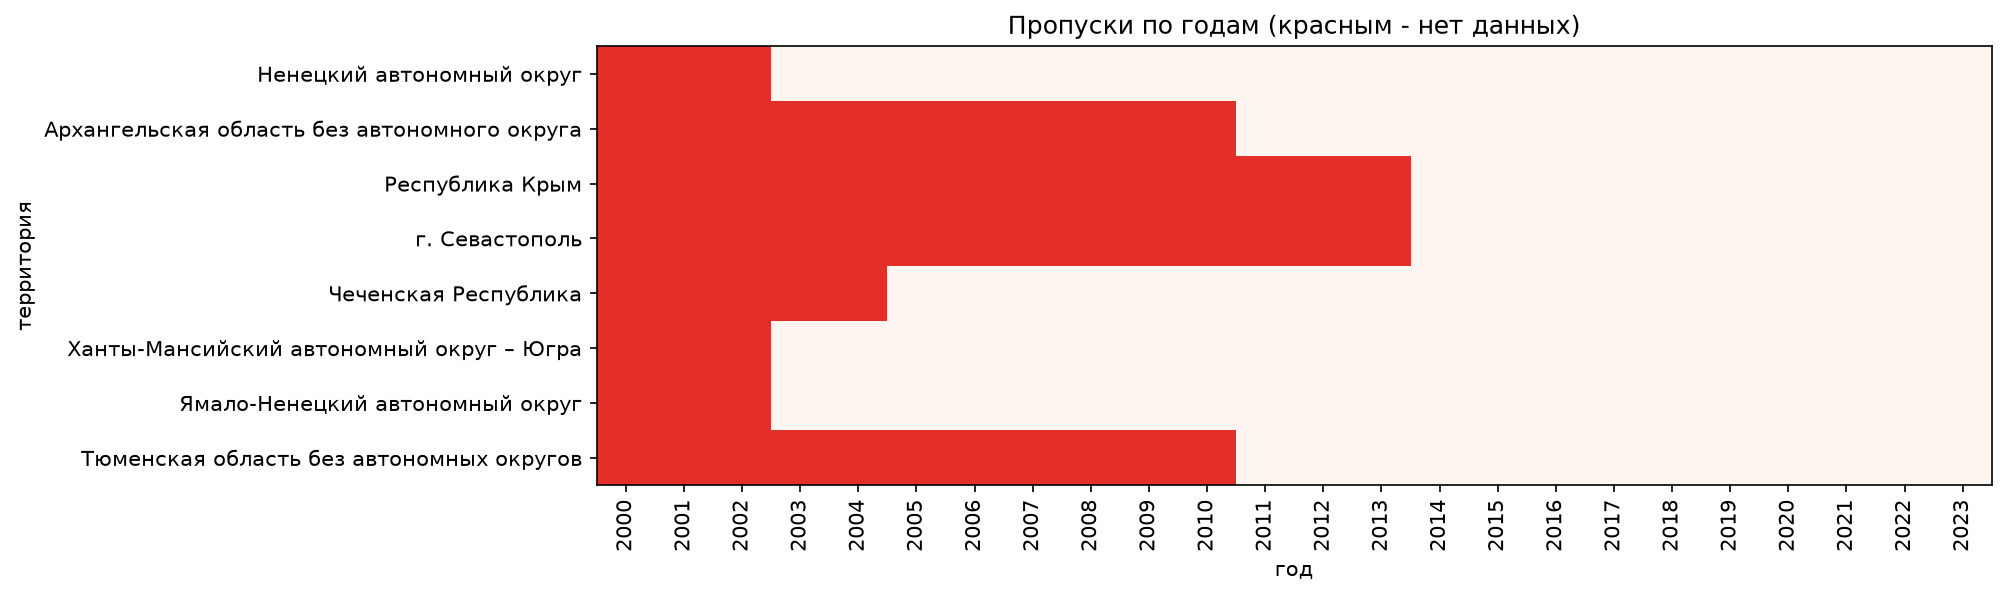
\includegraphics[width=\textwidth]{01_missing.png}
    \caption{Пропуски по годам: красным отмечены годы без данных}
    \label{fig:missing}
\end{figure}

Пропуски все "с начала ряда": 

- у Крыма и Севастополя нет 2000-2013 (данные с 2014 года)

- у двух строк "без автономного округа" нет 2000-2010, 

- у Чечни 2000-2004, 

- у трёх автономных округов (НАО, ХМАО, ЯНАО) 2000-2002. 

Внутри остальных рядов пропусков нет. По таске "длительные начальные фрагменты" не восстанавливаем - все эти позиции выбрасываем

\clearpage
\section{Исключённые территории}

Из 96 строк дропаем 17(табл.~\ref{tab:excluded}) : 

- строка по РФ

- 8 федеральных округов

- 2 дублирующих агрегата

- 6 субъектов с неполным рядом. 

Архангельская и Тюменская области в файле даны вместе с автономными округами, а сами АО отдельно выкинуты из-за неполного ряда, так что двойного счёта не остаётся. 
К слову, у Южного и Северо-Кавказского ФО значение за 2000 год подозрительно большое (около 96 и 76 тыс. руб. при 15-20 тыс. у их же регионов), но они и так исключены.

Для анализа остаётся 79 субъектов с полным рядом 2000--2023.

\begin{table}[H]
\centering
\caption{Исключённые территории и причины исключения}
\label{tab:excluded}
\small
\begin{tabular}{p{8.2cm}p{7.8cm}}
\toprule
Территория & Причина \\
\midrule
Российская Федерация (строка <<--- всего>>) & агрегат по стране \\
Центральный, Северо-Западный, Южный, Северо-Кавказский, Приволжский, Уральский, Сибирский, Дальневосточный ФО (8 строк) & агрегаты по федеральным округам \\
Архангельская область без автономного округа & дублирующий агрегат, нет данных за 2000--2010 \\
Тюменская область без автономных округов & дублирующий агрегат, нет данных за 2000--2010 \\
Республика Крым & неполный ряд, нет данных за 2000--2013 \\
г. Севастополь & неполный ряд, нет данных за 2000--2013 \\
Чеченская Республика & неполный ряд, нет данных за 2000--2004 \\
Ненецкий автономный округ & неполный ряд, нет данных за 2000--2002 \\
Ханты-Мансийский автономный округ -- Югра & неполный ряд, нет данных за 2000--2002 \\
Ямало-Ненецкий автономный округ & неполный ряд, нет данных за 2000--2002 \\
\bottomrule
\end{tabular}
\end{table}

Архангельская и Тюменская области в файле даны вместе с автономными округами, а сами АО отдельно выкинуты из-за неполного ряда, так что двойного счёта не остаётся. К слову, у Южного и Северо-Кавказского ФО значение за 2000 год подозрительно большое (около 96 и 76 тыс. руб. при 15--20 тыс. у их же регионов), но они и так исключены.

\section{Перевод в длинный формат и ряды по регионам}

Через \texttt{melt} таблица переводится в длинный формат <<регион --- год --- значение>>: 96 строк $\times$ 24 года дают 2304 строки, после фильтра остаётся 1896 (79 регионов $\times$ 24 года). Дальше из этого собирается отдельный ряд на каждый регион с годовым индексом (\texttt{PeriodIndex}, его понимают и \texttt{statsmodels}, и \texttt{sktime}), а для признаков все ряды ещё сложены в одну таблицу <<год $\times$ регион>>.

\section{Точечные аномалии}

Пропуски обработали, но хорошо бы проверить одиночные выбросы. Считаю отклонение логарифма от среднего соседних лет: для гладко растущего ряда оно небольшое, выбросы сходу будут видны

\begin{figure}[H]
    \centering
    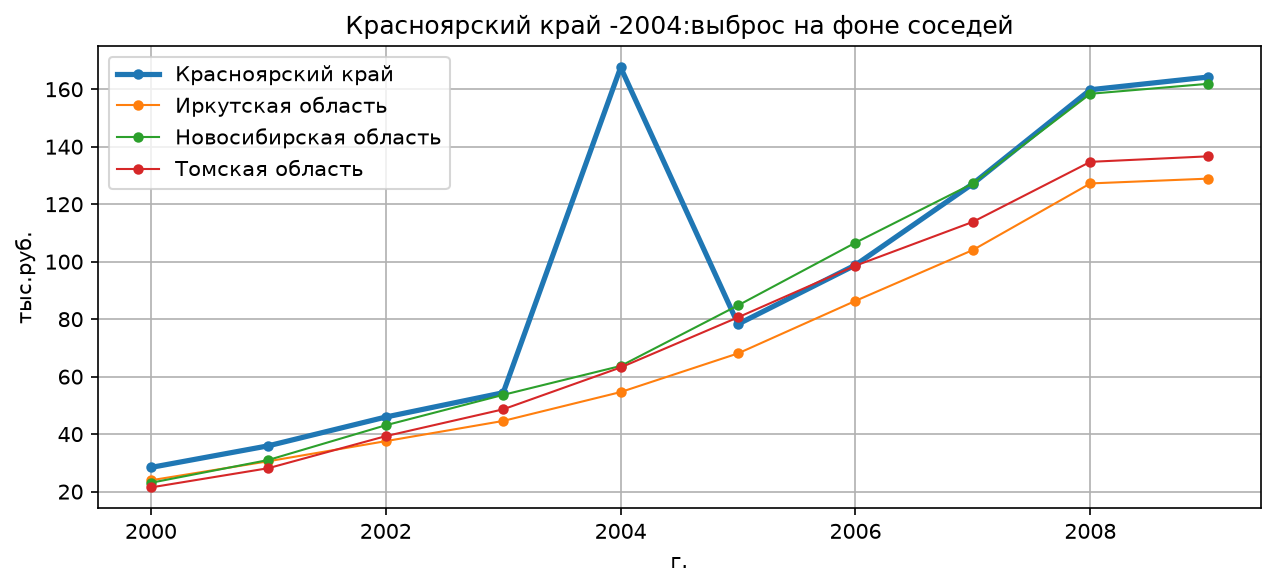
\includegraphics[width=0.8\textwidth]{02_krasnoyarsk_spike.png}
    \caption{Красноярский край, 2004 год: точечный выброс на фоне соседних регионов}
    \label{fig:spike}
\end{figure}

Красноярский край в 2004 году --- какой-то явный косяк в данных: 54.4 -> 167.6 -> 78.3 тыс. руб., то есть рост в 3 раза и сразу падение вдвое (рис.~\ref{fig:spike}). Если предположить, что там лишняя единичка в начале числа, получается 67.6 тыс., и это хорошо ложится в траекторию. Остальные отклонения сильно меньше, это обычные колебания.

Как фиксил: эту точку внутри ряда заменил средним геометрическим соседей (65.3 тыс.). Это не восстановление длинного куска, так что условию не противоречит. Без этого признак <<максимальное годовое падение>> у Красноярска был бы $-53\%$, и он стал бы отдельным кластером из одного региона.

\section{Общая картина}

\begin{figure}[H]
    \centering
    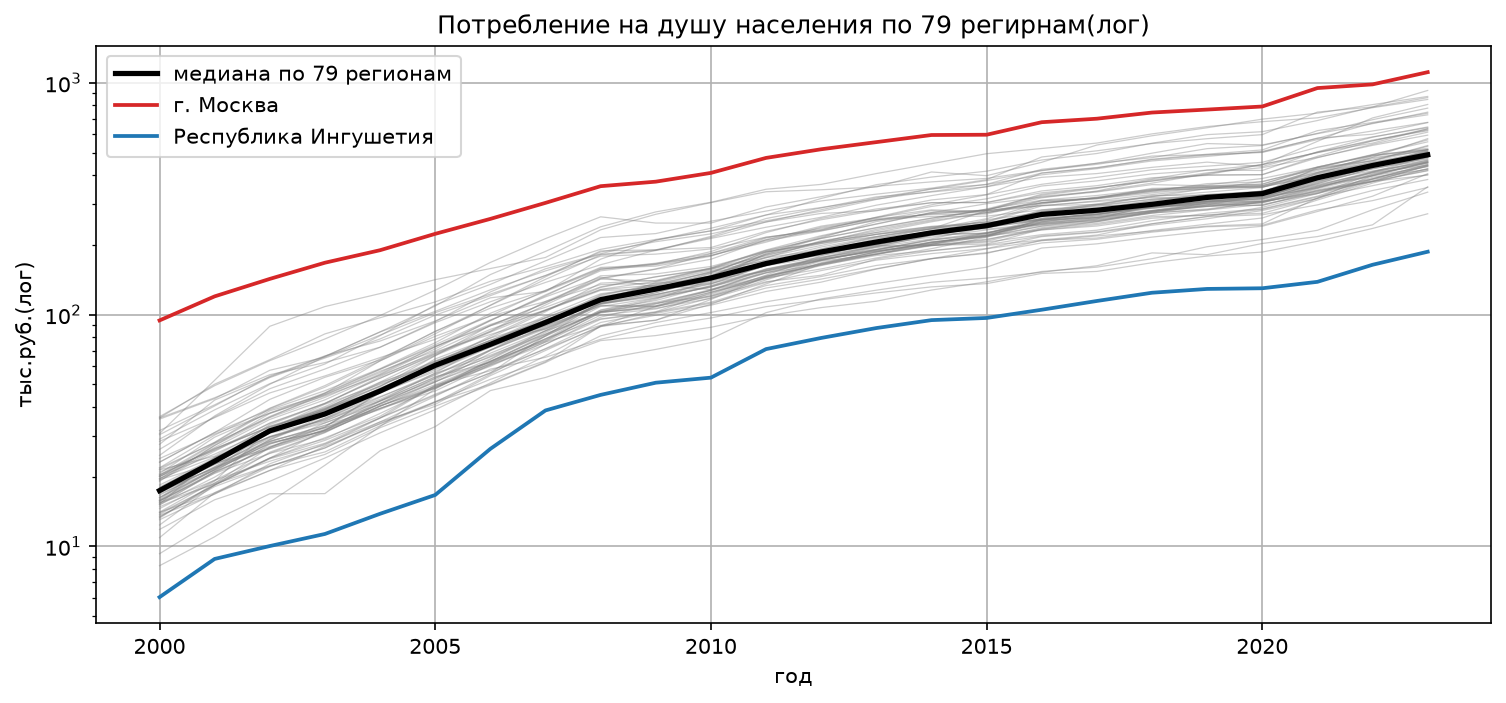
\includegraphics[width=\textwidth]{03_all_regions.png}
    \caption{Потребление на душу населения по 79 регионам, логарифмическая шкала}
    \label{fig:all}
\end{figure}

Все 79 рядов растут почти параллельно (рис.~\ref{fig:all}). Медиана за 23 года выросла с 17.4 до 489 тыс. руб., то есть в 28 раз. Это текущие цены, так что большая часть этого роста --- инфляция. Поэтому корректно сравнивать регионы между собой внутри одного года, а не, например, Курск 2023 года с Курском 2000-го.

Разброс уровней огромный. Москва в 2000 году была выше медианы в 5.4 раза (94.4 против 17.4 тыс.), к 2023 разрыв сжался до 2.3 раза (1111 против 489), т.е. регионы догоняли столицу. Ингушетия всё время внизу: 6 тыс. в 2000 и 187 тыс. в 2023.

На медиане видны изломы --- 2009, 2015 и 2020 годы, где рост резко замедляется (медианный темп 9.1\%, 6.9\% и 3.8\% против 25--26\% в 2004--2008), а после 2020 снова разгон до 12--15\% в год.

Я в своё время писал диплом по мировому кризису 2008 года (стартовал он в 2007 как пузырь на рынке недвижимости в США), поэтому 2009 тут логичен --- с лагом примерно в год. До <<моей>> Беларуси он вообще докатился только к 2011. В 2014 обвалилась цена на нефть (и как следствие курс рубля), частично ещё санкции после Крыма, а до потребителей это докатилось к 2015. Ну а 2020 год --- это, естественно, пандемия.

% =======Этап 2



\chapter{Кластерный анализ регионов}

\section{Признаки рядов}

Ряды в текущих ценах, поэтому абсолютные величины в основном говорят про масштаб и инфляцию, а не про характер динамики. Признаки считал по рекомендованному списку из задания (табл.~\ref{tab:features}). Пара уточнений: средний годовой темп роста считаю как CAGR, а <<максимальное годовое падение>> --- это минимальный годовой темп, и он вполне может быть положительным.

\begin{table}[H]
\centering
\caption{Признаки временных рядов}
\label{tab:features}
\small
\begin{tabular}{lp{7.5cm}c}
\toprule
Признак & Что показывает & В модели \\
\midrule
mean & средний уровень потребления за период & как лог(средн.) \\
cv & коэффициент вариации std/mean, волатильность без масштаба & да \\
cagr & средний годовой темп роста $(y_{2023}/y_{2000})^{1/23}-1$ & да \\
total\_change & отношение $y_{2023}/y_{2000}$ & нет \\
max\_drop & минимальный годовой темп роста (худший год) & да \\
neg\_share & доля лет со снижением к предыдущему году & да \\
\bottomrule
\end{tabular}
\end{table}

\begin{figure}[H]
    \centering
    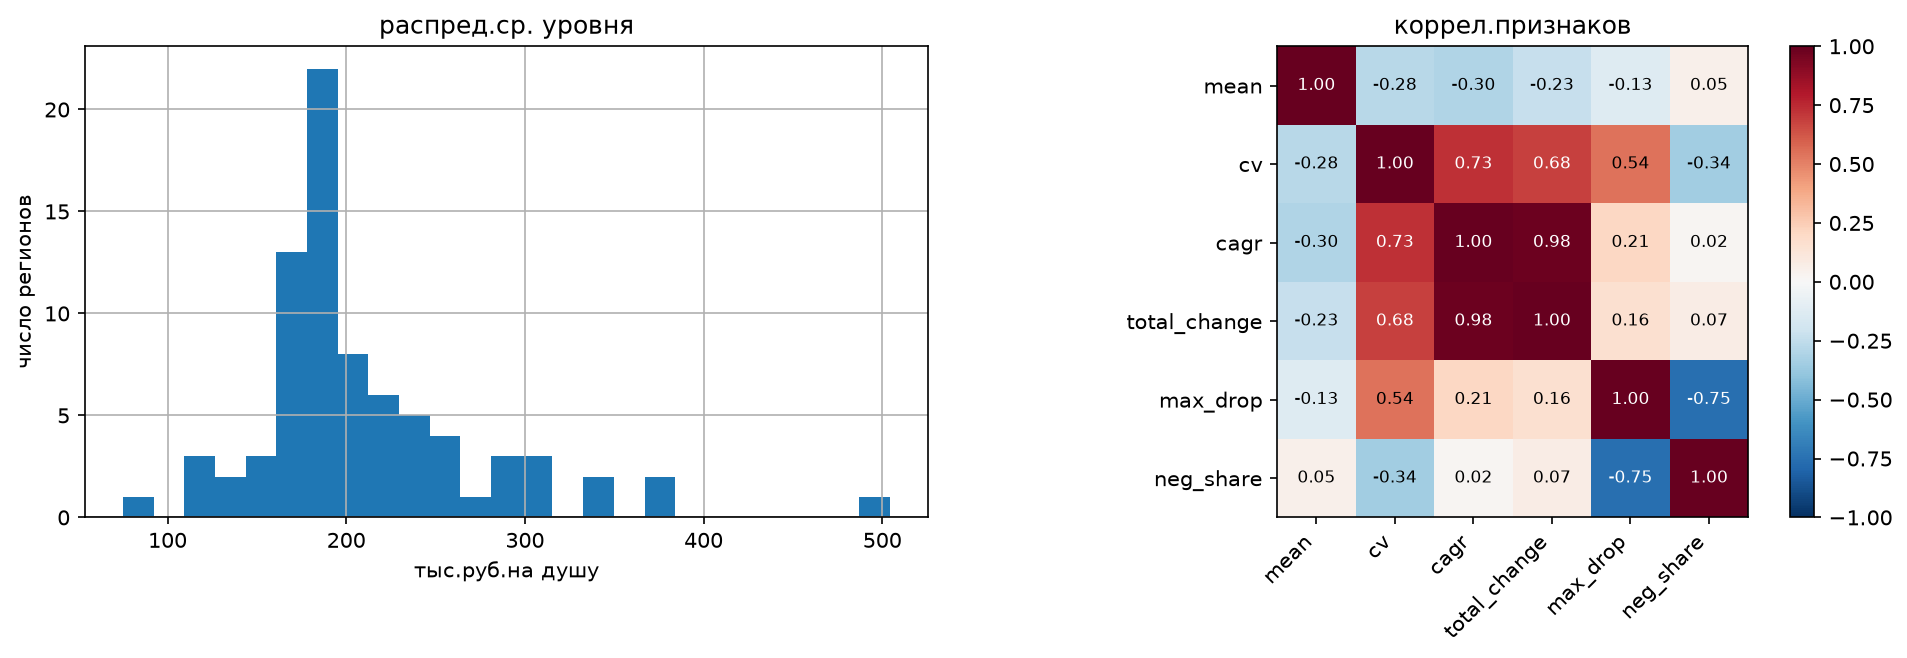
\includegraphics[width=\textwidth]{04_features.png}
    \caption{Распределение среднего уровня и корреляции признаков}
    \label{fig:features}
\end{figure}

Средний уровень сильно скошен вправо, асимметрия 1.69 (рис.~\ref{fig:features}). Основная масса регионов в районе 170--230 тыс., а дальше хвост. В ноутбуке вывел топ-20 по среднему уровню: после Москвы (504 тыс.) идут Сахалин (372), Чукотка (370), Санкт-Петербург (341), Магаданская область (335), Тюменская область (313), Якутия (309), Камчатка (306), Мурманская область (294), и т.д. --- северные и сырьевые регионы плюс две столицы. В k-means с евклидовым расстоянием такой хвост легко перетягивает на себя отдельный кластер, поэтому уровень беру в логарифме. Асимметрия падает до 0.16 (рис.~\ref{fig:logmean}).

\begin{figure}[H]
    \centering
    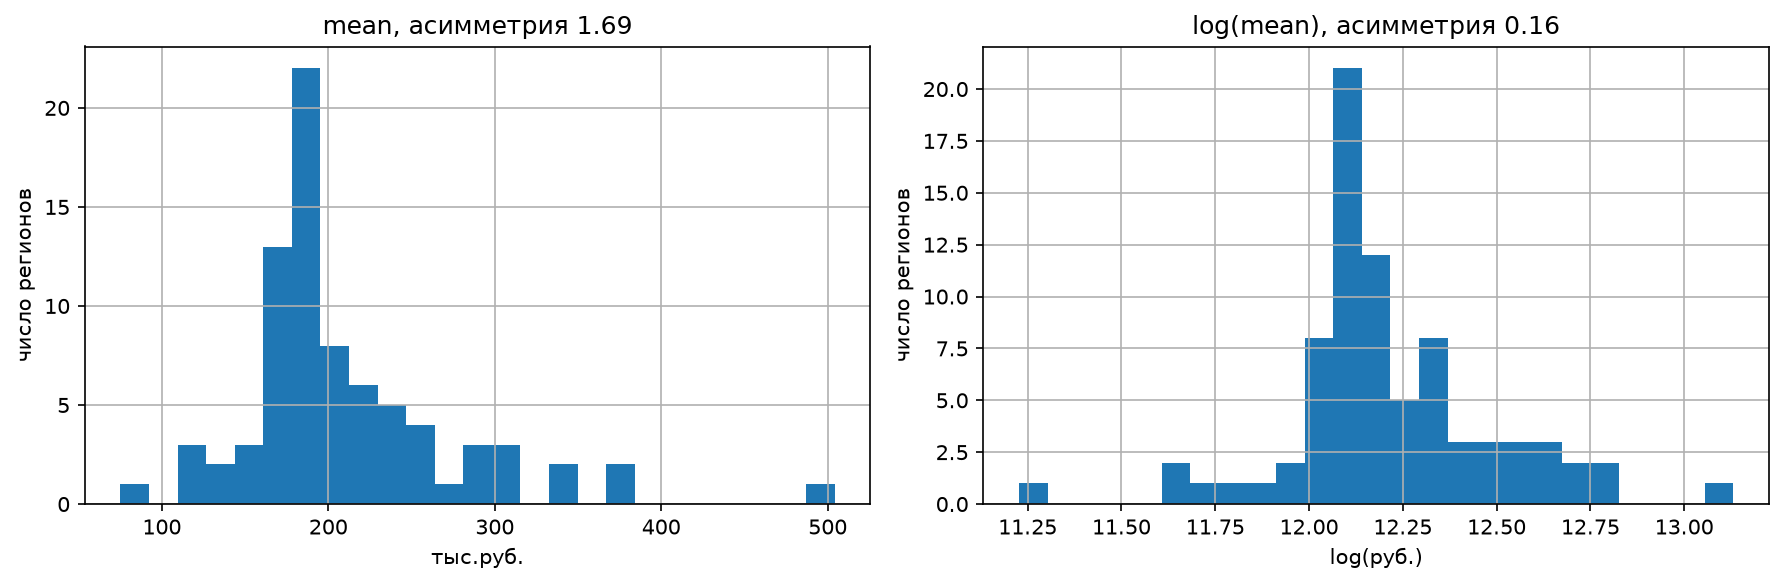
\includegraphics[width=\textwidth]{04b_log_mean.png}
    \caption{Распределение среднего уровня до и после логарифмирования}
    \label{fig:logmean}
\end{figure}

total\_change выкидываю: с cagr корреляция 0.98, что логично --- $\text{total\_change}=(1+\text{cagr})^{23}$, одна и та же величина в другой шкале. С ней темп роста считался бы в расстоянии дважды. cv тоже связан с cagr (0.73): чем быстрее рос регион, тем сильнее разъезжаются начало и конец ряда. Но он несёт ещё и информацию о форме траектории, так что оставляю.

Итого пять признаков: log(mean), cv, cagr, max\_drop и neg\_share, из них четыре относительные и от масштаба экономики не зависят. Перед кластеризацией все они стандартизированы \texttt{StandardScaler} --- единицы разные (логарифм рублей, доли), и без этого K-means смотрел бы только на самый <<широкий>> признак.

\section{Выбор алгоритма и числа кластеров}

Беру K-means. Признаков мало, все числовые и после стандартизации в одной шкале, регионов 79 --- для такого случая это самый простой вариант. Плюс центроиды сразу дают профиль кластера и <<самый типичный>> регион, а он понадобится на этапе 3. \texttt{n\_init=50}, чтобы результат не зависел от неудачной инициализации, и \texttt{random\_state=42} для воспроизводимости.

\begin{table}[H]
\centering
\caption{Silhouette score для разного числа кластеров}
\label{tab:silhouette}
\begin{tabular}{crrl}
\toprule
k & Silhouette & Inertia & Размеры кластеров \\
\midrule
2 & 0.406 & 259.6 & 58, 21 \\
3 & 0.321 & 205.1 & 45, 18, 16 \\
4 & 0.268 & 169.2 & 31, 28, 14, 6 \\
\bottomrule
\end{tabular}
\end{table}

\begin{figure}[H]
    \centering
    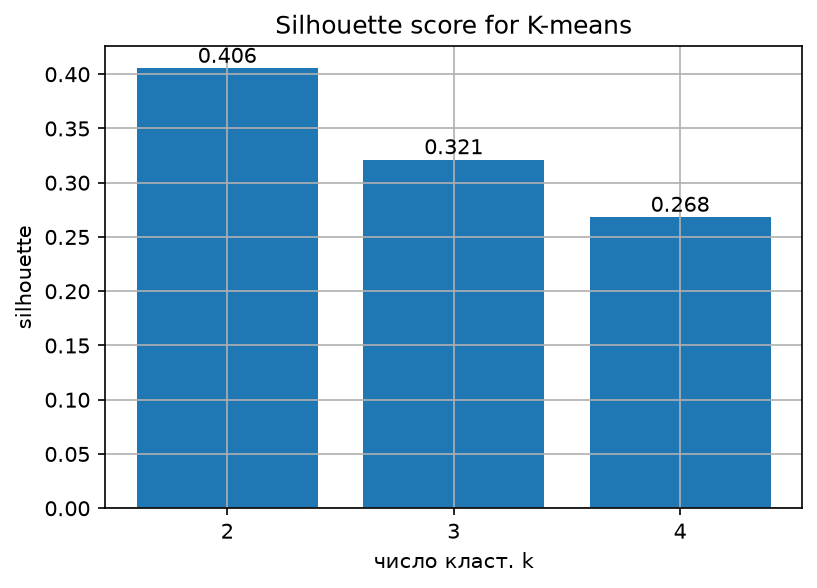
\includegraphics[width=0.55\textwidth]{05_silhouette.png}
    \caption{Silhouette score для K-means при k = 2, 3, 4}
    \label{fig:silhouette}
\end{figure}

\begin{table}[H]
\centering
\caption{Профили кластеров при k = 2, 3, 4 (средние по кластеру)}
\label{tab:profiles_k}
\small
\begin{tabular}{cccrrrrrr}
\toprule
k & Кластер & n & mean, тыс. руб. & cv & cagr, \% & total\_change & max\_drop, \% & neg\_share, \% \\
\midrule
2 & 0 & 21 & 232.7 & 0.68 & 15.17 & 26.9 & $-2.17$ & 4.14 \\
  & 1 & 58 & 201.8 & 0.73 & 15.68 & 28.9 & 2.75 & 0.00 \\
\midrule
3 & A & 45 & 198.2 & 0.74 & 16.01 & 30.7 & 3.08 & 0.00 \\
  & B & 18 & 216.4 & 0.69 & 15.58 & 28.7 & $-2.44$ & 4.59 \\
  & C & 16 & 235.8 & 0.67 & 14.20 & 21.5 & 1.18 & 0.27 \\
\midrule
4 & 0 & 14 & 205.3 & 0.70 & 16.01 & 31.0 & $-1.83$ & 4.66 \\
  & 1 & 31 & 210.2 & 0.75 & 16.25 & 32.1 & 3.35 & 0.00 \\
  & 2 & 28 & 194.3 & 0.70 & 15.00 & 25.1 & 1.98 & 0.00 \\
  & 3 & 6 & 292.9 & 0.62 & 13.37 & 18.4 & $-3.36$ & 3.62 \\
\bottomrule
\end{tabular}
\end{table}

По силуэту лучший вариант k = 2 (0.406), дальше 0.321 и 0.268 для k = 3 и 4 (табл.~\ref{tab:silhouette}). Но если смотреть профили (табл.~\ref{tab:profiles_k}), k = 2 делит регионы по сути по одному признаку: были ли вообще годы со снижением (21 регион) или нет (58). Это правда, но маловато --- внутри большой группы оказываются и Москва с её 11\% роста в год, и Краснодарский край с 17.5\%.

При k = 3 из <<беспросадочной>> группы выделяются 16 регионов с высоким стартом и заметно более медленным ростом (cagr 14.2\% против 16.0\%, рост за период в 21.5 раза против 30.7). Появляется вторая содержательная ось --- догоняющий рост против уже высокого уровня. k = 4 силуэт роняет ещё ниже и делает две вещи: дробит <<устойчивый рост>> на чуть быстрее и чуть медленнее (16.3\% против 15.0\%) и выделяет 6 регионов --- Москва, Самарская и Тюменская области, Пермский край, Кузбасс, Якутия, --- где смешаны высокий уровень и просадки. Интерпретировать это уже сложнее. Так что беру k = 3: силуэт не максимальный, но положительный и заметный, а группы нормально читаются экономически.

\section{Описание кластеров}

Номера кластеров у K-means произвольные, поэтому имена в коде даются по профилю: кластер с максимальной долей лет снижения --- B, из оставшихся тот, у которого cagr меньше, --- C, последний --- A.

\begin{table}[H]
\centering
\caption{Итоговые кластеры (k = 3)}
\label{tab:clusters}
\small
\resizebox{\textwidth}{!}{%
\begin{tabular}{lrrrrrrrr}
\toprule
Кластер & n & mean, тыс. руб. & cv & cagr, \% & max\_drop, \% & neg\_share, \% & 2000, тыс. руб. (медиана) & 2023, тыс. руб. (медиана) \\
\midrule
A: устойчивый быстрый рост & 45 & 198.2 & 0.74 & 16.01 & 3.08 & 0.00 & 16.2 & 479.1 \\
B: рост с просадками & 18 & 216.4 & 0.69 & 15.58 & $-2.44$ & 4.59 & 17.9 & 477.3 \\
C: высокий старт, медленный рост & 16 & 235.8 & 0.67 & 14.20 & 1.18 & 0.27 & 23.5 & 519.6 \\
\bottomrule
\end{tabular}}
\end{table}

\begin{table}[H]
\centering
\caption{Состав кластеров}
\label{tab:cluster_lists}
\small
\begin{tabular}{p{3.2cm}p{12.8cm}}
\toprule
Кластер & Регионы \\
\midrule
A: устойчивый быстрый рост (45) & Амурская, Архангельская, Белгородская, Брянская, Владимирская, Волгоградская, Ивановская, Калининградская, Калужская, Кировская, Костромская, \textbf{Курская}, Ленинградская, Липецкая, Магаданская, Московская, Нижегородская, Оренбургская, Орловская, Пензенская, Псковская, Рязанская, Саратовская, Сахалинская, Тверская, Тульская, Ульяновская, Ярославская области; Еврейская АО; Краснодарский край; республики Адыгея, Алтай, Бурятия, Ингушетия, Карелия, Марий Эл, Мордовия, Северная Осетия -- Алания, Татарстан, Тыва, Хакасия, Кабардино-Балкарская, Удмуртская, Чувашская; г. Санкт-Петербург \\
\midrule
B: рост с просадками (18) & Воронежская, Кемеровская, Курганская, Омская, \textbf{Ростовская}, Свердловская, Тамбовская, Тюменская, Челябинская области; Алтайский, Забайкальский, Пермский, Приморский, Ставропольский края; республики Дагестан, Калмыкия, Саха (Якутия); Чукотский АО \\
\midrule
C: высокий старт, медленный рост (16) & Астраханская, Вологодская, Иркутская, Мурманская, Новгородская, Новосибирская, Самарская, Смоленская, Томская области; Камчатский, \textbf{Красноярский}, Хабаровский края; республики Башкортостан, Коми, Карачаево-Черкесская; г. Москва \\
\bottomrule
\end{tabular}
\end{table}

\textbf{A: устойчивый быстрый рост} (45 регионов). Ни одного года со снижением за 23 года, даже худший год в среднем +3.1\%. Средний темп 16.0\% в год, рост за период в 30.7 раза. Стартовали с самого низкого уровня (медиана 16.2 тыс. в 2000) и к 2023 догнали остальных (479 тыс.). Сюда попала большая часть Центра и Поволжья, Ингушетия, КБР, Северная Осетия, Санкт-Петербург, Краснодарский край. По сути это догоняющие регионы без сильной привязки к сырью и тяжёлой промышленности: кризисы они проходили замедлением, но не падением.

\textbf{B: рост с просадками} (18 регионов). Средний темп почти такой же, 15.6\%, но в среднем около одного года со снижением (4.6\% лет), худший --- $-2.4\%$. Снижения приходятся на кризисы: в 2009 снижались 4 региона кластера, в 2015 --- 4, в 2020 --- 6 (табл.~\ref{tab:neg_years}). Сюда попал Урал (Свердловская, Челябинская, Кемеровская, Тюменская области, Пермский край), Приморье, Якутия, Чукотка, Забайкалье, а с юга Ростовская область, Ставрополье, Дагестан и Калмыкия. Металлургия, уголь, нефть и экспорт --- всё это сильнее реагирует на кризисы.

\textbf{C: высокий старт, медленный рост} (16 регионов). В 2000 году медиана 23.5 тыс., на 45\% выше, чем у A, а рост за период всего в 21.5 раза (14.2\% в год). Снижений почти нет (одно, в 2015). В 2023 эти регионы всё ещё самые <<богатые>> (медиана 520 тыс.), но отрыв заметно меньше. Тут Москва, Самарская область, Коми, Мурманск, Красноярский край, Иркутская, Новосибирская и Томская области, Хабаровск, Камчатка --- крупные, северные или сырьевые регионы, которым догонять было некого. Пара регионов попала сюда скорее из-за медленного роста, чем из-за уровня: Карачаево-Черкесия и Смоленская область.

\begin{table}[H]
\centering
\caption{Число регионов со снижением показателя по годам}
\label{tab:neg_years}
\begin{tabular}{lrrrrrr}
\toprule
Кластер & 2009 & 2010 & 2015 & 2018 & 2019 & 2020 \\
\midrule
A: устойчивый быстрый рост & 0 & 0 & 0 & 0 & 0 & 0 \\
B: рост с просадками & 4 & 1 & 4 & 1 & 3 & 6 \\
C: высокий старт, медленный рост & 0 & 0 & 1 & 0 & 0 & 0 \\
\bottomrule
\end{tabular}
\end{table}

\begin{figure}[H]
    \centering
    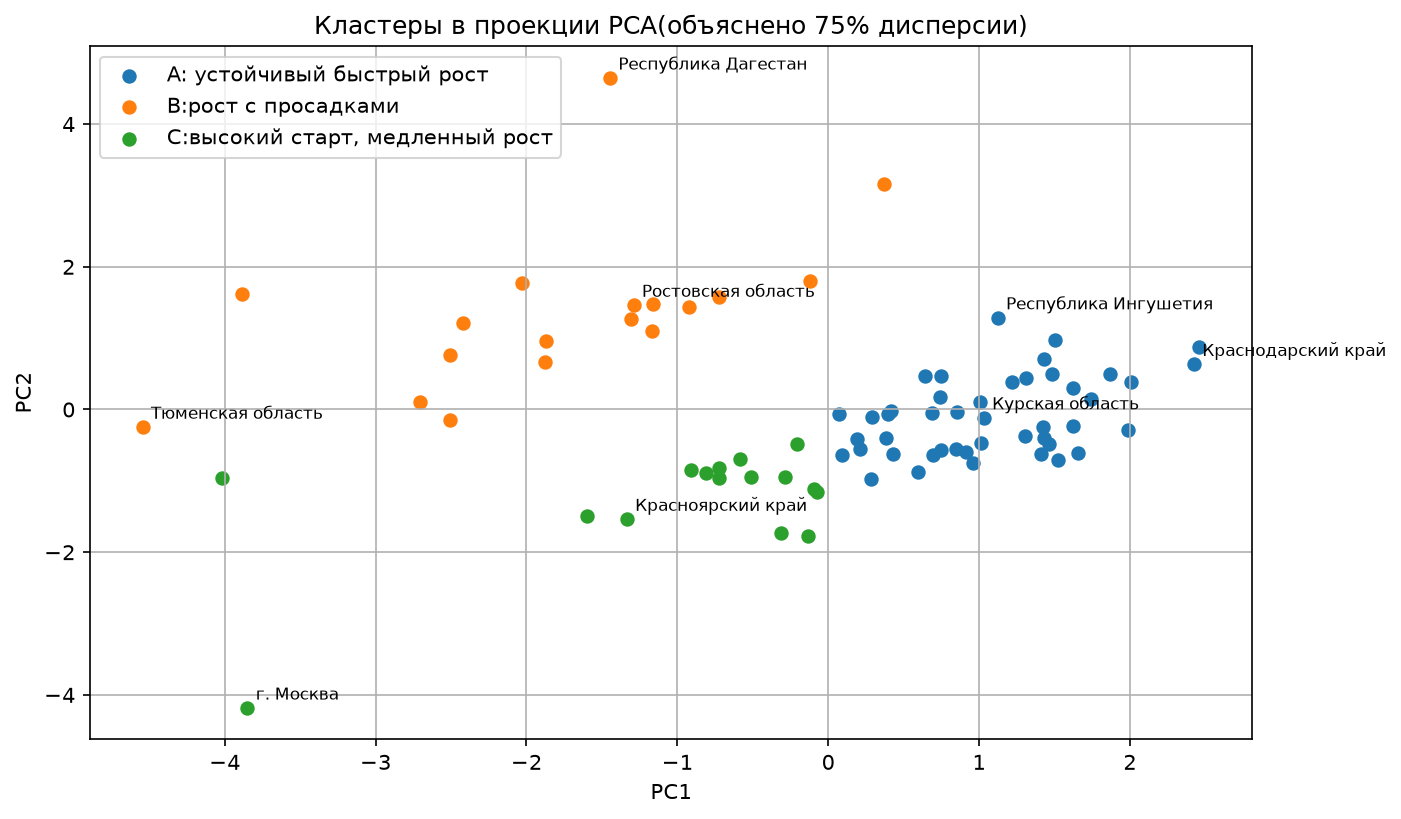
\includegraphics[width=0.85\textwidth]{06_clusters_pca.png}
    \caption{Кластеры в проекции на две главные компоненты}
    \label{fig:pca}
\end{figure}

На PCA-проекции (две компоненты объясняют 75\% дисперсии, рис.~\ref{fig:pca}) кластеры разделяются довольно чисто. Ось PC1 --- это по сути <<скорость и гладкость роста>> (нагрузки cv 0.56, max\_drop 0.53, cagr 0.41 против neg\_share $-0.43$), по ней A справа, B и C слева. PC2 разводит B и C: у B выше доля лет со снижением, у C ниже темп.

\begin{figure}[H]
    \centering
    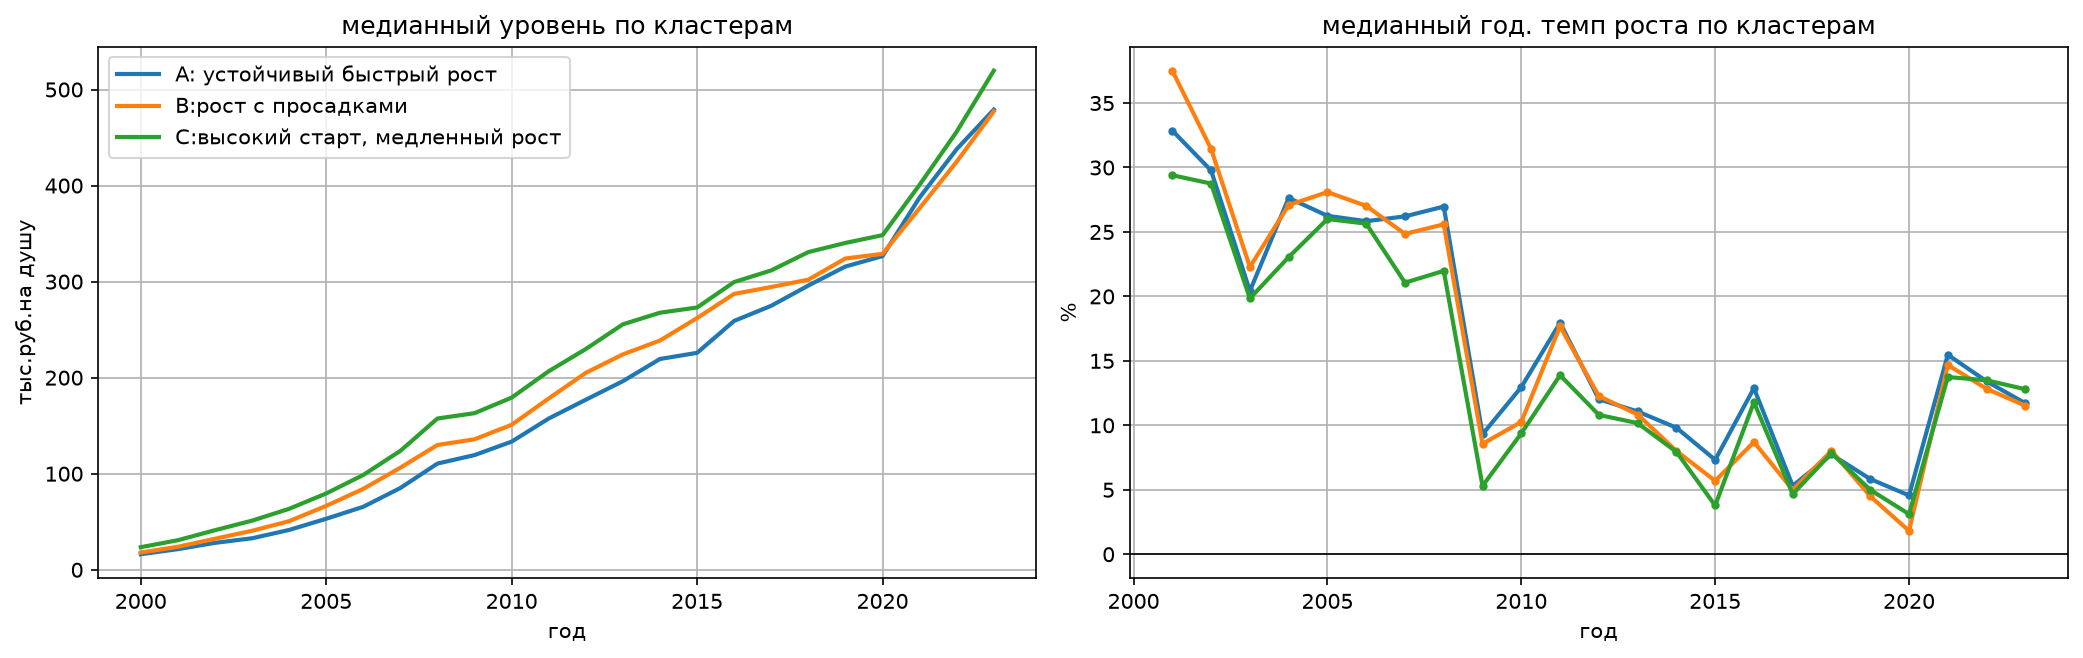
\includegraphics[width=\textwidth]{07_clusters_dynamics.png}
    \caption{Медианный уровень и медианный годовой темп роста по кластерам}
    \label{fig:cl_dyn}
\end{figure}

По медианам кластеров (рис.~\ref{fig:cl_dyn}) видно, что провалы 2009, 2015 и 2020 есть у всех трёх, разница в глубине и в стартовом уровне. У C медиана выше весь период, а темп почти каждый год до 2008 ниже, чем у A и B. У B в 2020 медианный темп падает до 2\%.

% =======ЭТАП 3 ======
\chapter{Выбор регионов для прогнозирования}

Кластеров три, значит берём по одному региону из каждого. Критерий --- репрезентативность: регион с минимальным расстоянием до центроида своего кластера в стандартизованном пространстве признаков, то есть тот, чьи признаки ближе всего к средним по кластеру (табл.~\ref{tab:candidates}).

\begin{table}[H]
\centering
\caption{Три ближайших к центроиду региона в каждом кластере}
\label{tab:candidates}
\begin{tabular}{llr}
\toprule
Кластер & Регион & Расстояние до центроида \\
\midrule
A & \textbf{Курская область} & \textbf{0.091} \\
  & Тверская область & 0.392 \\
  & Оренбургская область & 0.406 \\
\midrule
B & \textbf{Ростовская область} & \textbf{0.654} \\
  & Ставропольский край & 0.814 \\
  & Забайкальский край & 0.920 \\
\midrule
C & \textbf{Красноярский край} & \textbf{0.485} \\
  & Томская область & 0.706 \\
  & Новосибирская область & 0.832 \\
\bottomrule
\end{tabular}
\end{table}

\begin{table}[H]
\centering
\caption{Признаки выбранных регионов против средних по кластеру}
\label{tab:rep_vs_cluster}
\small
\begin{tabular}{lrrrrrr}
\toprule
 & mean, тыс. руб. & cv & cagr, \% & total\_change & max\_drop, \% & neg\_share, \% \\
\midrule
Курская область & 190.9 & 0.74 & 16.02 & 30.5 & 3.11 & 0.00 \\
среднее по A & 198.2 & 0.74 & 16.01 & 30.7 & 3.08 & 0.00 \\
\midrule
Ростовская область & 218.9 & 0.71 & 15.84 & 29.5 & $-2.04$ & 4.35 \\
среднее по B & 216.4 & 0.69 & 15.58 & 28.7 & $-2.44$ & 4.59 \\
\midrule
Красноярский край & 227.9 & 0.66 & 13.81 & 19.6 & 0.49 & 0.00 \\
среднее по C & 235.8 & 0.67 & 14.20 & 21.5 & 1.18 & 0.27 \\
\bottomrule
\end{tabular}
\end{table}

\textbf{Курская область} --- самый типичный регион кластера A и вообще всего набора: расстояние до центроида 0.09, признаки почти совпадают со средними по кластеру (cagr 16.02\% против 16.01\%, cv 0.74, ни одного года со снижением, табл.~\ref{tab:rep_vs_cluster}). Это эталон <<спокойного>> догоняющего роста.

\textbf{Ростовская область} ближе всех к центру кластера B (0.65). Один год снижения --- 2009, $-2.0\%$ (в среднем по B $-2.4\%$), темп 15.8\% против 15.6\%.

\textbf{Красноярский край} --- ближайший к центру C (0.49): рост за период в 19.6 раза при среднем по кластеру 21.5, темп 13.8\% против 14.2\%. Сырьевой регион с высоким стартом (в 2000 году 163\% от медианы). Единственный нюанс --- у него исправлена одна точка 2004 года, но она далеко от теста и на прогноз не влияет.

\begin{table}[H]
\centering
\caption{Базовая статистика выбранных регионов, 2000--2023}
\label{tab:base_stats}
\small
\resizebox{\textwidth}{!}{%
\begin{tabular}{lrrrrrr}
\toprule
Регион & Среднее, тыс. руб. & Мин. (год), тыс. руб. & Макс. (год), тыс. руб. & Наклон лин. тренда, тыс. руб./год & $R^2$ & Темп по лог-тренду, \%/год \\
\midrule
Курская область & 190.9 & 15.7 (2000) & 478.0 (2023) & 19.58 & 0.97 & 15.1 \\
Ростовская область & 218.9 & 19.3 (2000) & 567.0 (2023) & 21.68 & 0.96 & 14.3 \\
Красноярский край & 227.9 & 28.4 (2000) & 556.3 (2023) & 20.88 & 0.97 & 12.6 \\
\bottomrule
\end{tabular}}
\end{table}

По базовой статистике (табл.~\ref{tab:base_stats}) у всех трёх минимум в 2000 и максимум в 2023, ряды растут почти монотонно. Линейный тренд даёт наклон 19.6, 21.7 и 20.9 тыс. руб. в год с $R^2$ 0.96--0.97, но высокий $R^2$ тут обманчив: рост на самом деле экспоненциальный, и в процентах (тренд по логарифму) это 15.1\%, 14.3\% и 12.6\% в год.

% ============ этап 4
\chapter{Анализ выбранных регионов}

\section{Тренд и циклические колебания}

Тренд выделяю двумя способами, как и просили в задании: скользящим средним за 3 года~\cite{habr-ods} и фильтром Ходрика--Прескотта. HP считаю по логарифму ряда --- рост близок к экспоненциальному, и тогда циклическая компонента читается как отклонение от тренда в процентах. $\lambda = 100$ --- стандартное значение для годовых данных.

\begin{figure}[H]
    \centering
    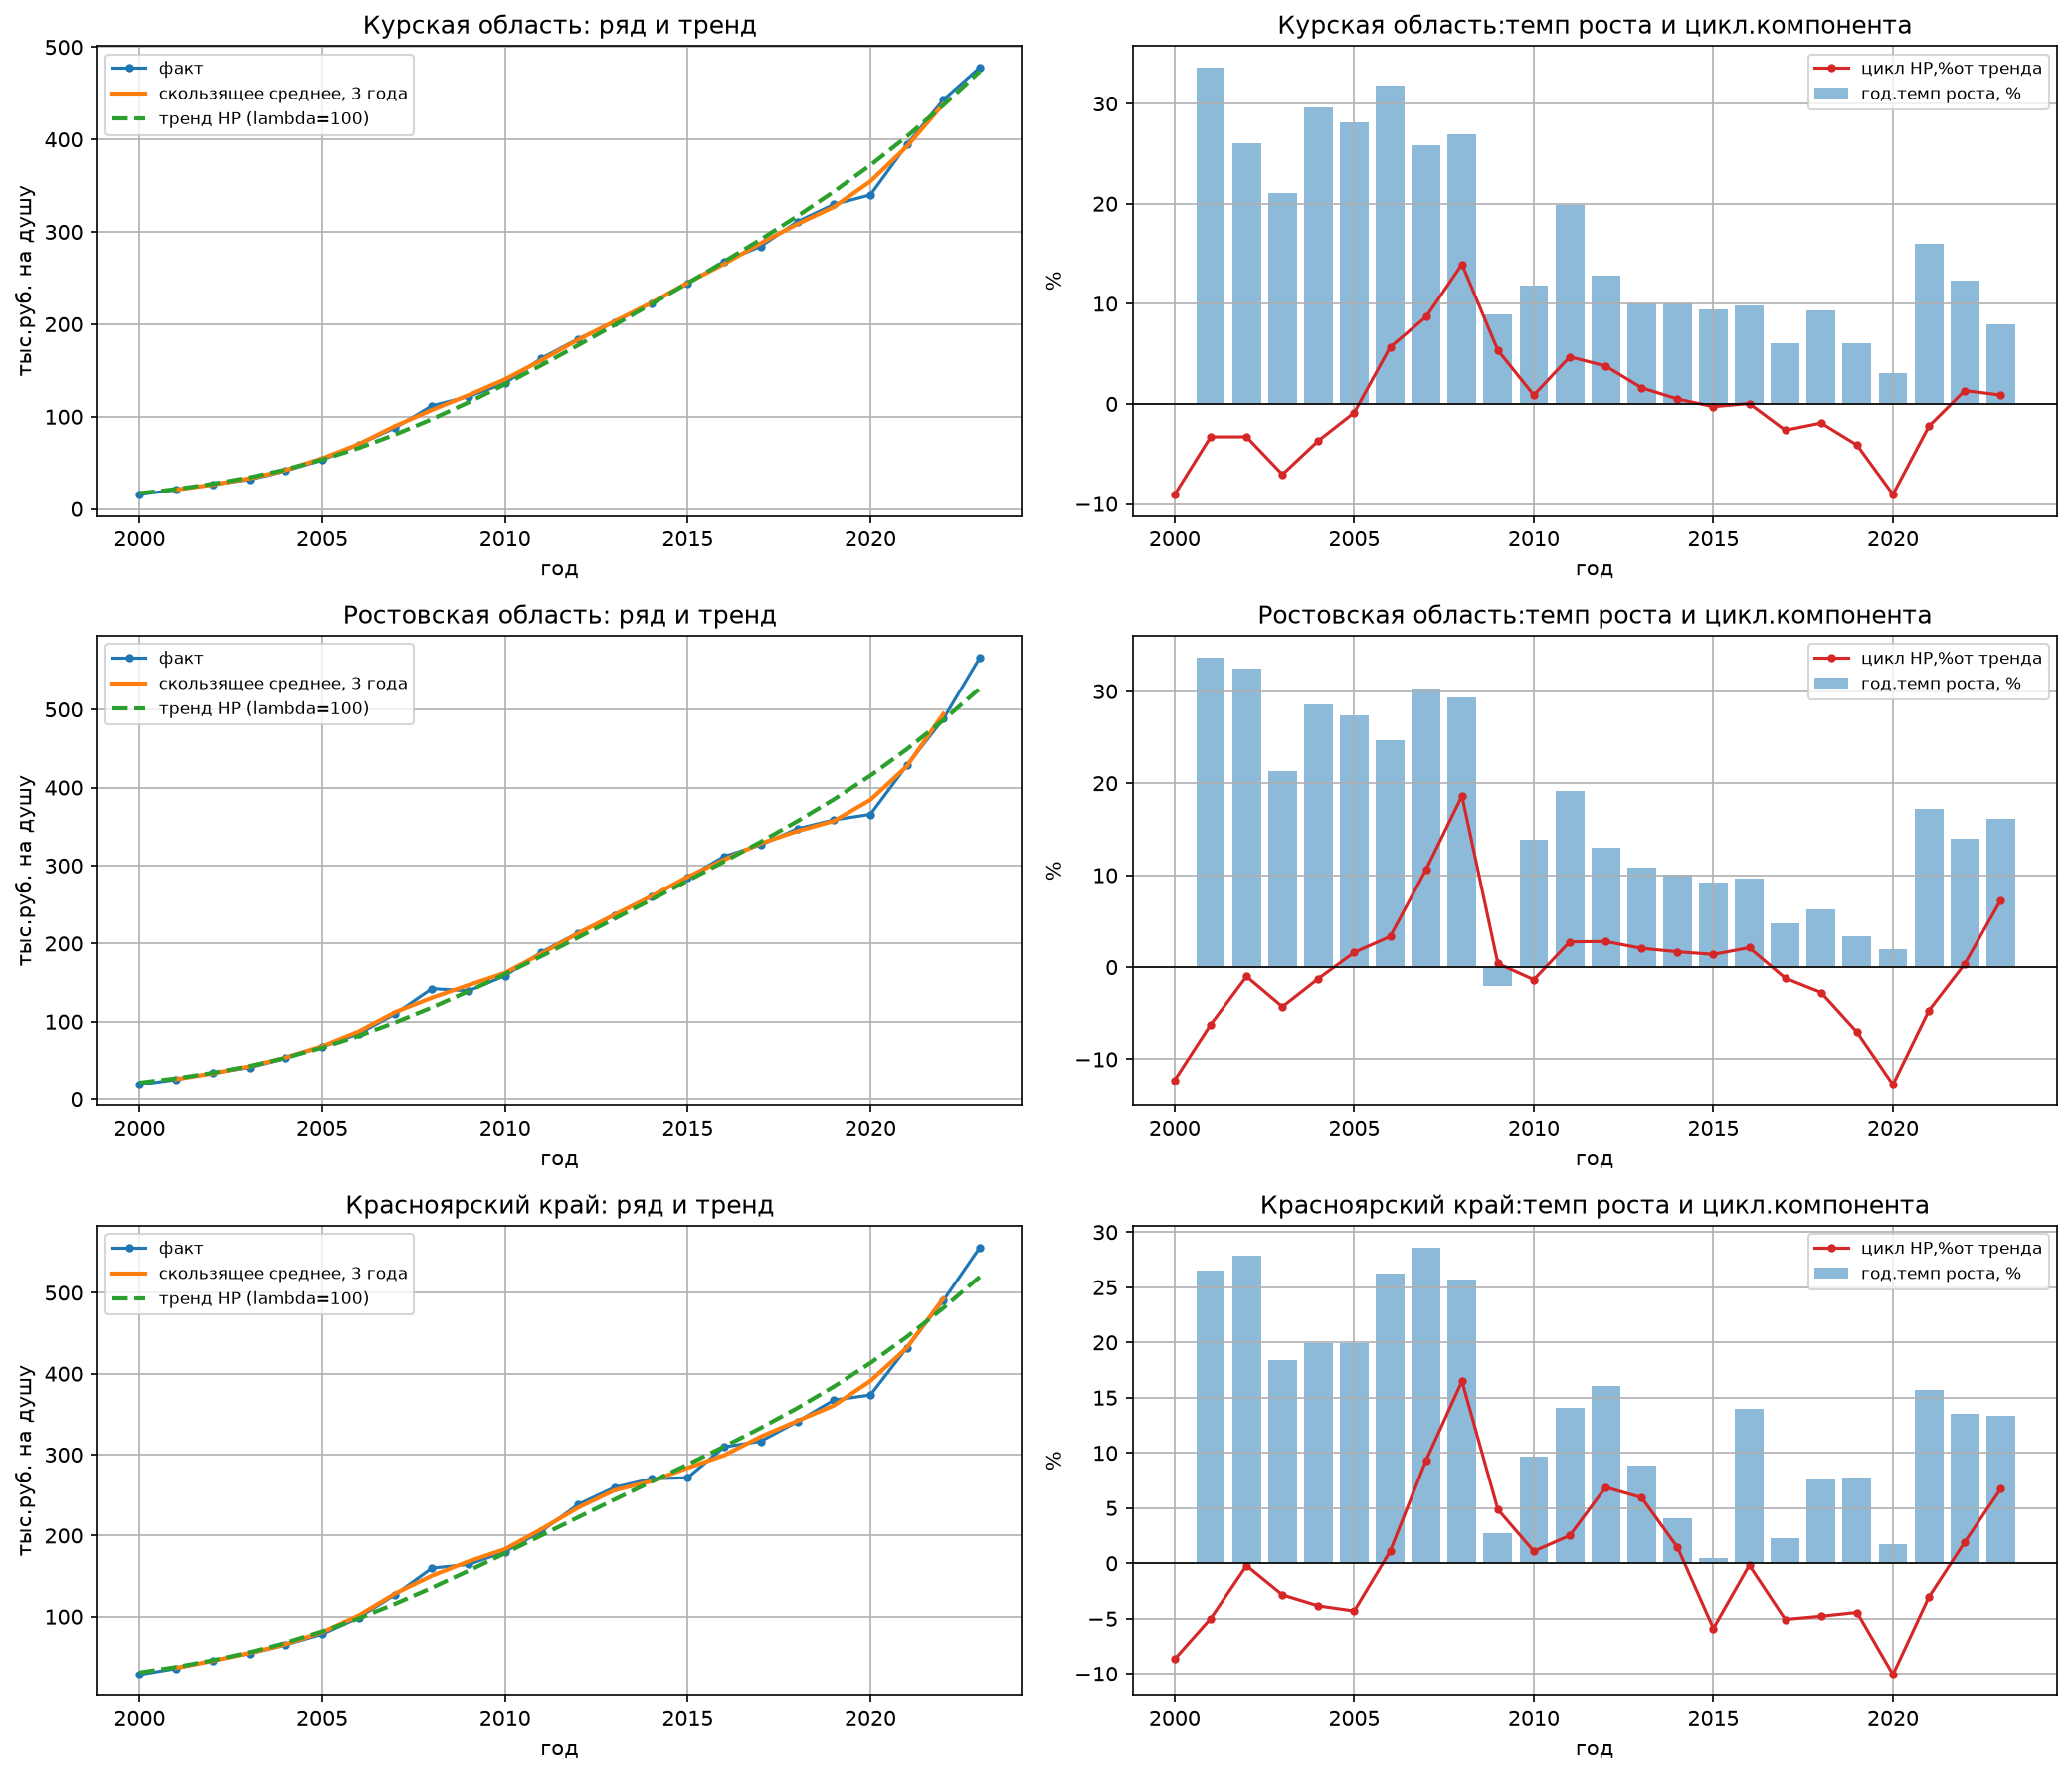
\includegraphics[width=\textwidth]{08_trend_cycle.png}
    \caption{Слева: ряд, скользящее среднее и HP-тренд. Справа: годовой темп роста и циклическая компонента HP}
    \label{fig:trend}
\end{figure}

\begin{table}[H]
\centering
\caption{Годы с наибольшим отклонением от HP-тренда}
\label{tab:cycle}
\small
\begin{tabular}{lccccc}
\toprule
Регион & \#1 & \#2 & \#3 & \#4 & \#5 \\
\midrule
Курская область & 2008: +14.0\% & 2000: $-9.1\%$ & 2020: $-9.0\%$ & 2007: +8.7\% & 2003: $-7.0\%$ \\
Ростовская область & 2008: +18.6\% & 2020: $-12.8\%$ & 2000: $-12.3\%$ & 2007: +10.6\% & 2023: +7.3\% \\
Красноярский край & 2008: +16.5\% & 2020: $-10.1\%$ & 2007: +9.3\% & 2000: $-8.7\%$ & 2012: +6.9\% \\
\bottomrule
\end{tabular}
\end{table}

Тренд у всех трёх сильно выражен и нелинейный: кривая выпуклая, в рублях рост ускоряется (рис.~\ref{fig:trend}). Скользящее среднее за 3 года почти лежит на факте, HP сглаживает сильнее и хорошо показывает, где ряд уходит от тренда. А вот сам темп роста за 23 года сильно менялся: 18--35\% в год в 2001--2008, обвал в 2009 (от $-2\%$ у Ростова до 9\% у Курска), 10--20\% в 2010--2013, в основном 2--10\% в 2014--2020 и снова 12--17\% в 2021--2023.

Циклическая компонента у всех трёх одинаковой формы (табл.~\ref{tab:cycle}). Пик в 2008 (+14.0\%, +18.6\%, +16.5\% от тренда) --- перегрев перед кризисом, затем провал 2020 ($-9.0\%$, $-12.8\%$, $-10.1\%$) --- пандемия. Значения 2000 года ($-9$..$-12\%$) --- это в основном краевой эффект HP-фильтра, на концах ряда он ненадёжен. Сильнее всего колеблется Ростовская область, у неё же единственный год со снижением (2009). У Красноярского края видна своя просадка в 2015, когда рост за год был всего +0.5\%, а Курская область самая гладкая.

\section{Почему здесь нет сезонной декомпозиции}

Сезонной декомпозиции не может быть! Сезонность - это повторяющийся паттерн внутри года (зима/лето или какие-нибудь кварталы), а у нас одна точка на год, внутригодовой структуры в данных просто нет.

\section{Тест Дики--Фуллера}

Проверяю четыре варианта ряда: уровень и логарифм (в регрессию теста включены константа и тренд, раз ряд явно растёт), первую и вторую разности логарифма (только константа). Разность логарифма --- это по сути годовой темп роста. Число лагов подбирается по AIC, но не больше 3: в ряду всего 24 точки, а по умолчанию \texttt{adfuller} берёт до 8 лагов и съедает треть наблюдений.

\begin{table}[H]
\centering
\caption{Тест Дики--Фуллера (p-value, в скобках --- статистика ADF)}
\label{tab:adf}
\small
\begin{tabular}{lcccc}
\toprule
Регион & уровень (c+t) & log (c+t) & d1 log (c) & d2 log (c) \\
\midrule
Курская область & 0.994 ($-0.02$) & 0.466 ($-2.24$) & 0.238 ($-2.12$) & \textbf{0.000} ($-5.90$) \\
Ростовская область & 1.000 (1.15) & 0.251 ($-2.67$) & 0.082 ($-2.66$) & \textbf{0.000} ($-5.42$) \\
Красноярский край & 1.000 (0.89) & 0.410 ($-2.34$) & 0.089 ($-2.62$) & \textbf{0.000} ($-6.14$) \\
\midrule
Крит. значение 5\% & $-3.62$ & $-3.62$ & $-3.01$ & $-3.01$ / $-3.02$ \\
\bottomrule
\end{tabular}
\end{table}

В уровнях единичный корень очевиден (p 0.99--1.0), в логарифме с трендом тоже (p 0.25--0.47), т.е. ряд не просто <<экспонента плюс шум вокруг неё>> (табл.~\ref{tab:adf}). Первая разность логарифма, то есть годовой темп роста, у Курской области нестационарна (p = 0.24), а у Ростова и Красноярска p = 0.08--0.09: на 10\% мы бы единичный корень отвергли, на 5\% --- нет. И это по графикам понятно, сам темп роста дрейфует --- от 25--30\% в начале 2000-х к 5--10\% в конце 2010-х. Вторая разность логарифма стационарна у всех (p $<$ 0.001).

Поэтому для ARIMA d = 2 на логарифме. Оговорка тут есть: в ряду всего 24 точки, мощность ADF при такой длине маленькая, и d = 2 может оказаться передифференцированием. Отрицательная автокорреляция на первом лаге во второй разности (ниже, $-0.28$..$-0.34$) как раз типичный признак такого, но она в пределах доверительной полосы.

\section{ACF и PACF}

ACF и PACF строю для того ряда, который по ADF получился стационарным, то есть для второй разности логарифма. До 8 лагов --- больше при 22 точках смысла нет, PACF дальше просто шумит. Логика стандартная: q прикидываем по ACF, p по PACF, смотрим уже на стационарном ряде~\cite{habr-arima}.

\begin{figure}[H]
    \centering
    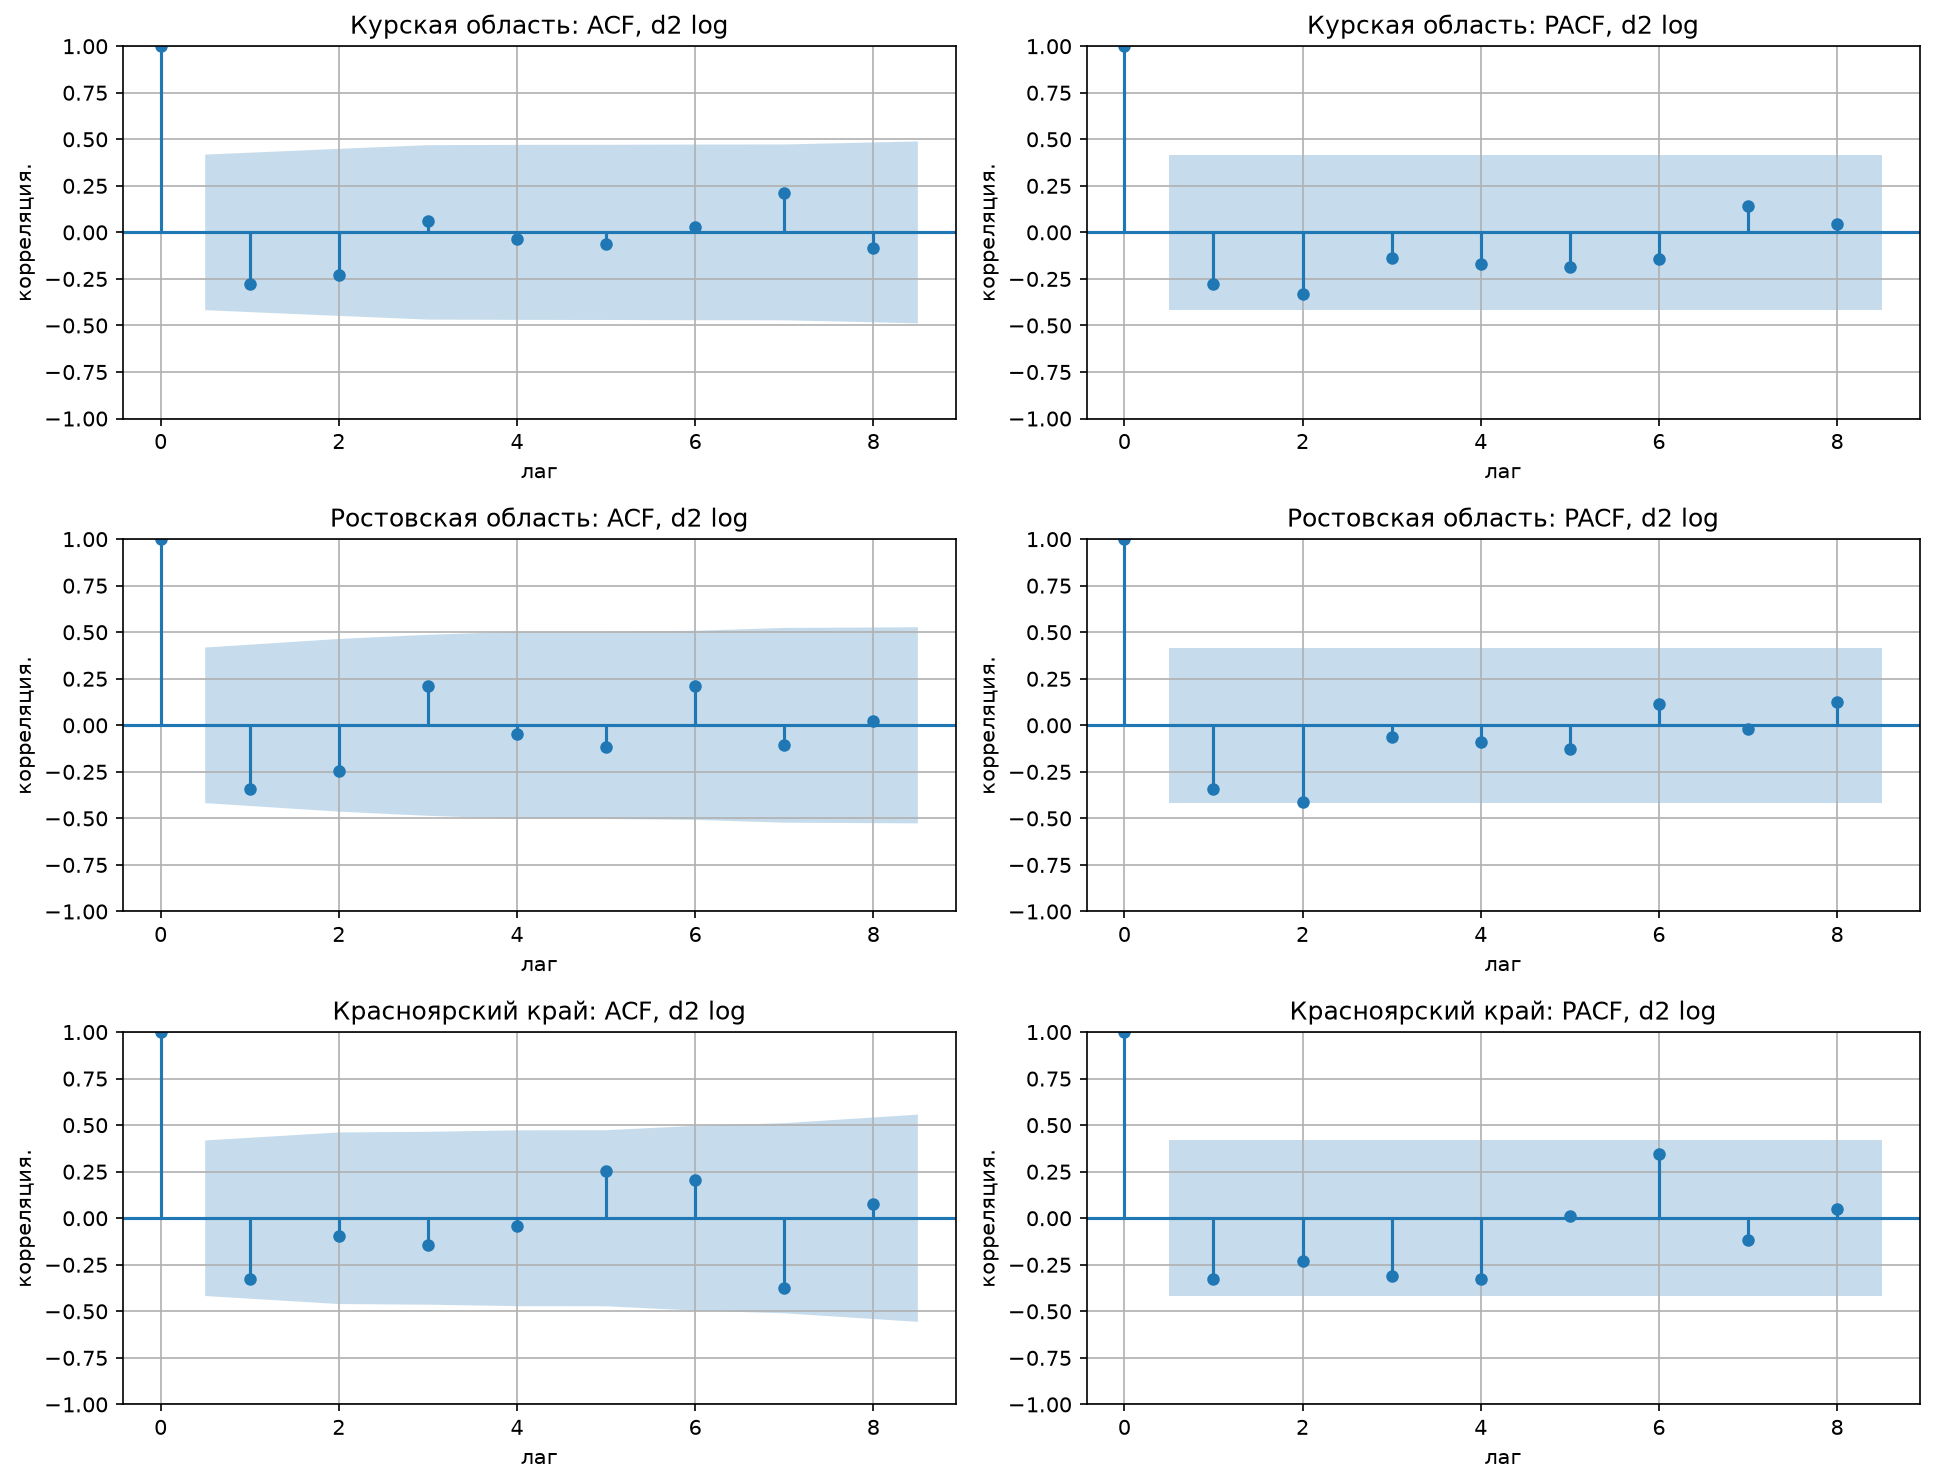
\includegraphics[width=\textwidth]{09_acf_pacf.png}
    \caption{ACF и PACF второй разности логарифма}
    \label{fig:acf}
\end{figure}

\begin{table}[H]
\centering
\caption{Значения ACF и PACF на первых лагах (граница значимости $\pm 0.42$)}
\label{tab:acf}
\small
\begin{tabular}{llrrrr}
\toprule
Регион & & лаг 1 & лаг 2 & лаг 3 & лаг 4 \\
\midrule
Курская область & ACF & $-0.28$ & $-0.23$ & 0.06 & $-0.04$ \\
 & PACF & $-0.28$ & $-0.33$ & $-0.14$ & $-0.17$ \\
Ростовская область & ACF & $-0.34$ & $-0.25$ & 0.21 & $-0.04$ \\
 & PACF & $-0.34$ & $-0.41$ & $-0.06$ & $-0.09$ \\
Красноярский край & ACF & $-0.33$ & $-0.10$ & $-0.15$ & $-0.04$ \\
 & PACF & $-0.33$ & $-0.23$ & $-0.31$ & $-0.32$ \\
\bottomrule
\end{tabular}
\end{table}

Все значения ACF и PACF у трёх регионов лежат внутри полосы $\pm 0.42$ (рис.~\ref{fig:acf}, табл.~\ref{tab:acf}), то есть формально вторая разность логарифма --- это белый шум. Отсюда базовая гипотеза \textbf{ARIMA(0,2,0)}: темп роста ведёт себя как случайное блуждание, прогноз = <<последний темп роста сохранится>>.

Но ACF на первом лаге у всех отрицательный ($-0.28$..$-0.34$) и дальше быстро затухает, а это картинка MA(1) с отрицательным коэффициентом --- поэтому вторая гипотеза \textbf{ARIMA(0,2,1)}. У Ростовской области PACF на втором лаге $-0.41$, почти на границе, так что для неё ещё вариант (2,2,0). У Красноярского края PACF на лагах 3--4 около $-0.32$, но при 21 точке я бы на это не опирался.

Итого жду p, q от 0 до 1, максимум 2. И ещё одно: ARIMA(0,2,1)--(0,2,2) теоретически очень близка к линейному Holt, так что на прогнозе Holt и ARIMA, скорее всего, разойдутся несильно.

\section{Сравнение регионов}

\begin{table}[H]
\centering
\caption{Сравнение выбранных регионов}
\label{tab:compare}
\small
\resizebox{\textwidth}{!}{%
\begin{tabular}{lrrrrrrrrr}
\toprule
Регион & Наклон, тыс. руб./год & CAGR, \% & CV & std темпа роста, п.п. & max\_drop, \% & std цикла HP, \% & ADF p (d1 log) & d & ACF лаг 1 \\
\midrule
Курская область & 19.58 & 16.02 & 0.737 & 9.44 & 3.11 & 5.34 & 0.238 & 2 & $-0.28$ \\
Ростовская область & 21.68 & 15.84 & 0.714 & 10.52 & $-2.04$ & 6.63 & 0.082 & 2 & $-0.34$ \\
Красноярский край & 20.88 & 13.81 & 0.659 & 8.96 & 0.49 & 6.19 & 0.089 & 2 & $-0.33$ \\
\bottomrule
\end{tabular}}
\end{table}

В рублях тренд круче всего у Ростовской области (21.7 тыс. руб. в год, табл.~\ref{tab:compare}), но в процентах быстрее всех росла Курская (cagr 16.0\%), а медленнее Красноярский край (13.8\%) --- он стартовал выше и растёт с большей базы. По волатильности лидирует Ростов: самый большой разброс темпа роста (10.5 п.п.) и цикла HP (6.6\%), и только у него есть год со снижением. У Красноярского края разброс темпа наименьший (9.0 п.п.), но цикл всё равно заметный (6.2\%) --- колебания у него более затяжные, через 2015 и 2020. Курская область самая ровная (цикл 5.3\%).

По стационарности все три одинаковые: нестационарны в уровнях, логарифмах и первых разностях на 5\%, стационарны во вторых разностях логарифма. Разница только в том, что у Ростова и Красноярска темп роста ближе к стационарному (p около 0.08--0.09 против 0.24 у Курска), то есть темп у них чаще возвращается к среднему после всплесков. ACF и PACF по форме похожи, отличия в деталях --- лаг 2 у Ростова и лаги 3--4 у Красноярска.

% ==этап5 ====================
\chapter{Прогнозирование}

\section{Разбиение, горизонт и модели}

Горизонт --- 5 лет, одинаковый для всех регионов. Тест --- последние 5 лет (2019--2023), train --- 2000--2018, это 19 из 24 точек, 79\%. Тот же горизонт 5 лет беру и для прогноза в будущее (2024--2028).

Модели:
\begin{itemize}
    \item \textbf{Naive} --- \texttt{NaiveForecaster(strategy="last")} из \texttt{sktime}, бейзлайн: прогноз = последнее значение~\cite{sf-m3};
    \item \textbf{Holt} --- экспоненциальное сглаживание с аддитивным трендом, оно же двойное экспоненциальное сглаживание: уровень плюс наклон~\cite{sf-m4,habr-ods}. В statsmodels это \texttt{ExponentialSmoothing} с \texttt{trend="add"};
    \item \textbf{ARIMA(p, d, q)}~\cite{sf-m5} --- d берётся из теста Дики--Фуллера (этап 4), p и q от 0 до 2 подбираются по AIC только на train.
\end{itemize}

Holt и ARIMA обучаются на логарифме ряда, прогноз потом возвращается через exp. Ряд в текущих ценах растёт почти по экспоненте, и в логарифме линейный тренд Holt означает постоянный темп роста, а не постоянный прирост в рублях --- для инфляционного ряда это естественнее. Метрики RMSE и MAPE считаются уже в рублях.

\begin{table}[H]
\centering
\caption{Подбор порядка ARIMA по AIC на train (лучшие три варианта)}
\label{tab:aic}
\begin{tabular}{lll}
\toprule
Курская область & Ростовская область & Красноярский край \\
\midrule
\textbf{(0,2,0)}: $-49.47$ & \textbf{(0,2,1)}: $-36.16$ & \textbf{(0,2,1)}: $-39.00$ \\
(0,2,1): $-48.91$ & (2,2,0): $-35.68$ & (0,2,0): $-38.09$ \\
(1,2,0): $-48.36$ & (0,2,2): $-34.19$ & (1,2,0): $-37.51$ \\
\bottomrule
\end{tabular}
\end{table}

Автоподбор по AIC подтвердил гипотезы с этапа 4 (табл.~\ref{tab:aic}). Для Курской области лучшей вышла ARIMA(0,2,0) --- чистый белый шум во второй разности, ровно базовая гипотеза. Для Ростова и Красноярска --- ARIMA(0,2,1), вторая гипотеза с отрицательным MA(1). У Ростова на втором месте (2,2,0), её тоже подсказывала PACF.

Разрыв по AIC с соседними вариантами маленький (0.5--0.9), при 19 точках AIC их толком не различает, но все топовые варианты лежат в ожидаемом диапазоне p, q от 0 до 2. Вообще ACF/PACF тут скорее дают стартовую точку, а окончательный порядок всё равно выбирается перебором --- в статье~\cite{habr-arima} автор пришла к тому же, только перебирала через optuna.

\section{Прогноз на тесте и метрики}

\begin{table}[H]
\centering
\caption{Метрики на тесте 2019--2023 (жирным --- лучшая модель)}
\label{tab:metrics}
\begin{tabular}{llrr}
\toprule
Регион & Модель & RMSE, руб. & MAPE, \% \\
\midrule
Курская область & Naive & 103\,408 & 20.0 \\
 & \textbf{Holt} & \textbf{13\,883} & \textbf{3.0} \\
 & ARIMA(0,2,0) & 16\,605 & 3.6 \\
\midrule
Ростовская область & Naive & 122\,816 & 19.0 \\
 & \textbf{Holt} & \textbf{39\,596} & \textbf{6.5} \\
 & ARIMA(0,2,1) & 41\,102 & 6.7 \\
\midrule
Красноярский край & Naive & 125\,731 & 21.3 \\
 & \textbf{Holt} & \textbf{45\,370} & \textbf{6.9} \\
 & ARIMA(0,2,1) & 46\,015 & 7.0 \\
\bottomrule
\end{tabular}
\end{table}

\begin{table}[H]
\centering
\caption{Ошибка по годам теста, (факт $-$ прогноз) / факт, \%}
\label{tab:test_errors}
\small
\begin{tabular}{llrrrrr}
\toprule
Регион & Модель & 2019 & 2020 & 2021 & 2022 & 2023 \\
\midrule
Курская область & Naive & 5.7 & 8.5 & 21.1 & 29.8 & 34.9 \\
 & Holt & $-2.5$ & $-8.0$ & $-1.2$ & 2.1 & 1.4 \\
 & ARIMA & $-3.2$ & $-9.4$ & $-3.2$ & $-0.5$ & $-1.9$ \\
\midrule
Ростовская область & Naive & 3.2 & 5.1 & 19.0 & 28.9 & 38.8 \\
 & Holt & $-3.8$ & $-9.1$ & 0.2 & 6.1 & 13.3 \\
 & ARIMA & $-3.6$ & $-8.8$ & 0.6 & 6.6 & 13.9 \\
\midrule
Красноярский край & Naive & 7.2 & 8.8 & 21.1 & 30.5 & 38.7 \\
 & Holt & 1.0 & $-3.8$ & 4.3 & 10.0 & 15.4 \\
 & ARIMA & 1.1 & $-3.7$ & 4.4 & 10.2 & 15.6 \\
\bottomrule
\end{tabular}
\end{table}

\begin{table}[H]
\centering
\caption{Holt на уровнях против Holt на логарифме, MAPE на тесте, \%}
\label{tab:holt_lvl}
\begin{tabular}{lrr}
\toprule
Регион & Holt на уровнях & Holt на логарифме \\
\midrule
Курская область & 6.0 & 3.0 \\
Ростовская область & 9.9 & 6.5 \\
Красноярский край & 10.2 & 6.9 \\
\bottomrule
\end{tabular}
\end{table}

Наивный прогноз проваливается везде: MAPE 19--21\%, к 2023 году <<замороженное>> значение 2018 отстаёт от факта на 35--39\% (табл.~\ref{tab:metrics}, \ref{tab:test_errors}). Ряд растёт, так что бейзлайн тут слабый, но обе статистические модели обыгрывают его в 3--7 раз по RMSE, значит прогнозы содержательные.

Holt лучший во всех трёх регионах: MAPE 3.0\% у Курска, 6.5\% у Ростова, 6.9\% у Красноярска. ARIMA отстаёт совсем чуть-чуть (3.6, 6.7, 7.0\%) --- как и ожидалось, ARIMA(0,2,1) по сути та же модель локального линейного тренда.

По годам картина у моделей одинаковая. В 2019--2020 они переоценивают (в 2020 до $-8$..$-9\%$ у Курска и Ростова), тут пандемия. С 2021 у Ростова и Красноярска пошла недооценка, к 2023 уже +13.3\% и +15.4\%: в 2021--2023 рост номинального потребления ускорился до 13--17\% в год, а train (2000--2018) заканчивается на замедлении, и модели этого разгона знать не могли. Курская область тут исключение, у неё 2022--2023 были спокойнее (12.3\% и 7.9\%), и ошибка к 2023 всего +1.4\%.

Заодно проверил решение про логарифм: тот же Holt на уровнях даёт MAPE 6.0\%, 9.9\% и 10.2\% против 3.0\%, 6.5\% и 6.9\% на логарифме (табл.~\ref{tab:holt_lvl}), так что переход к логарифму себя оправдал.

\begin{figure}[H]
    \centering
    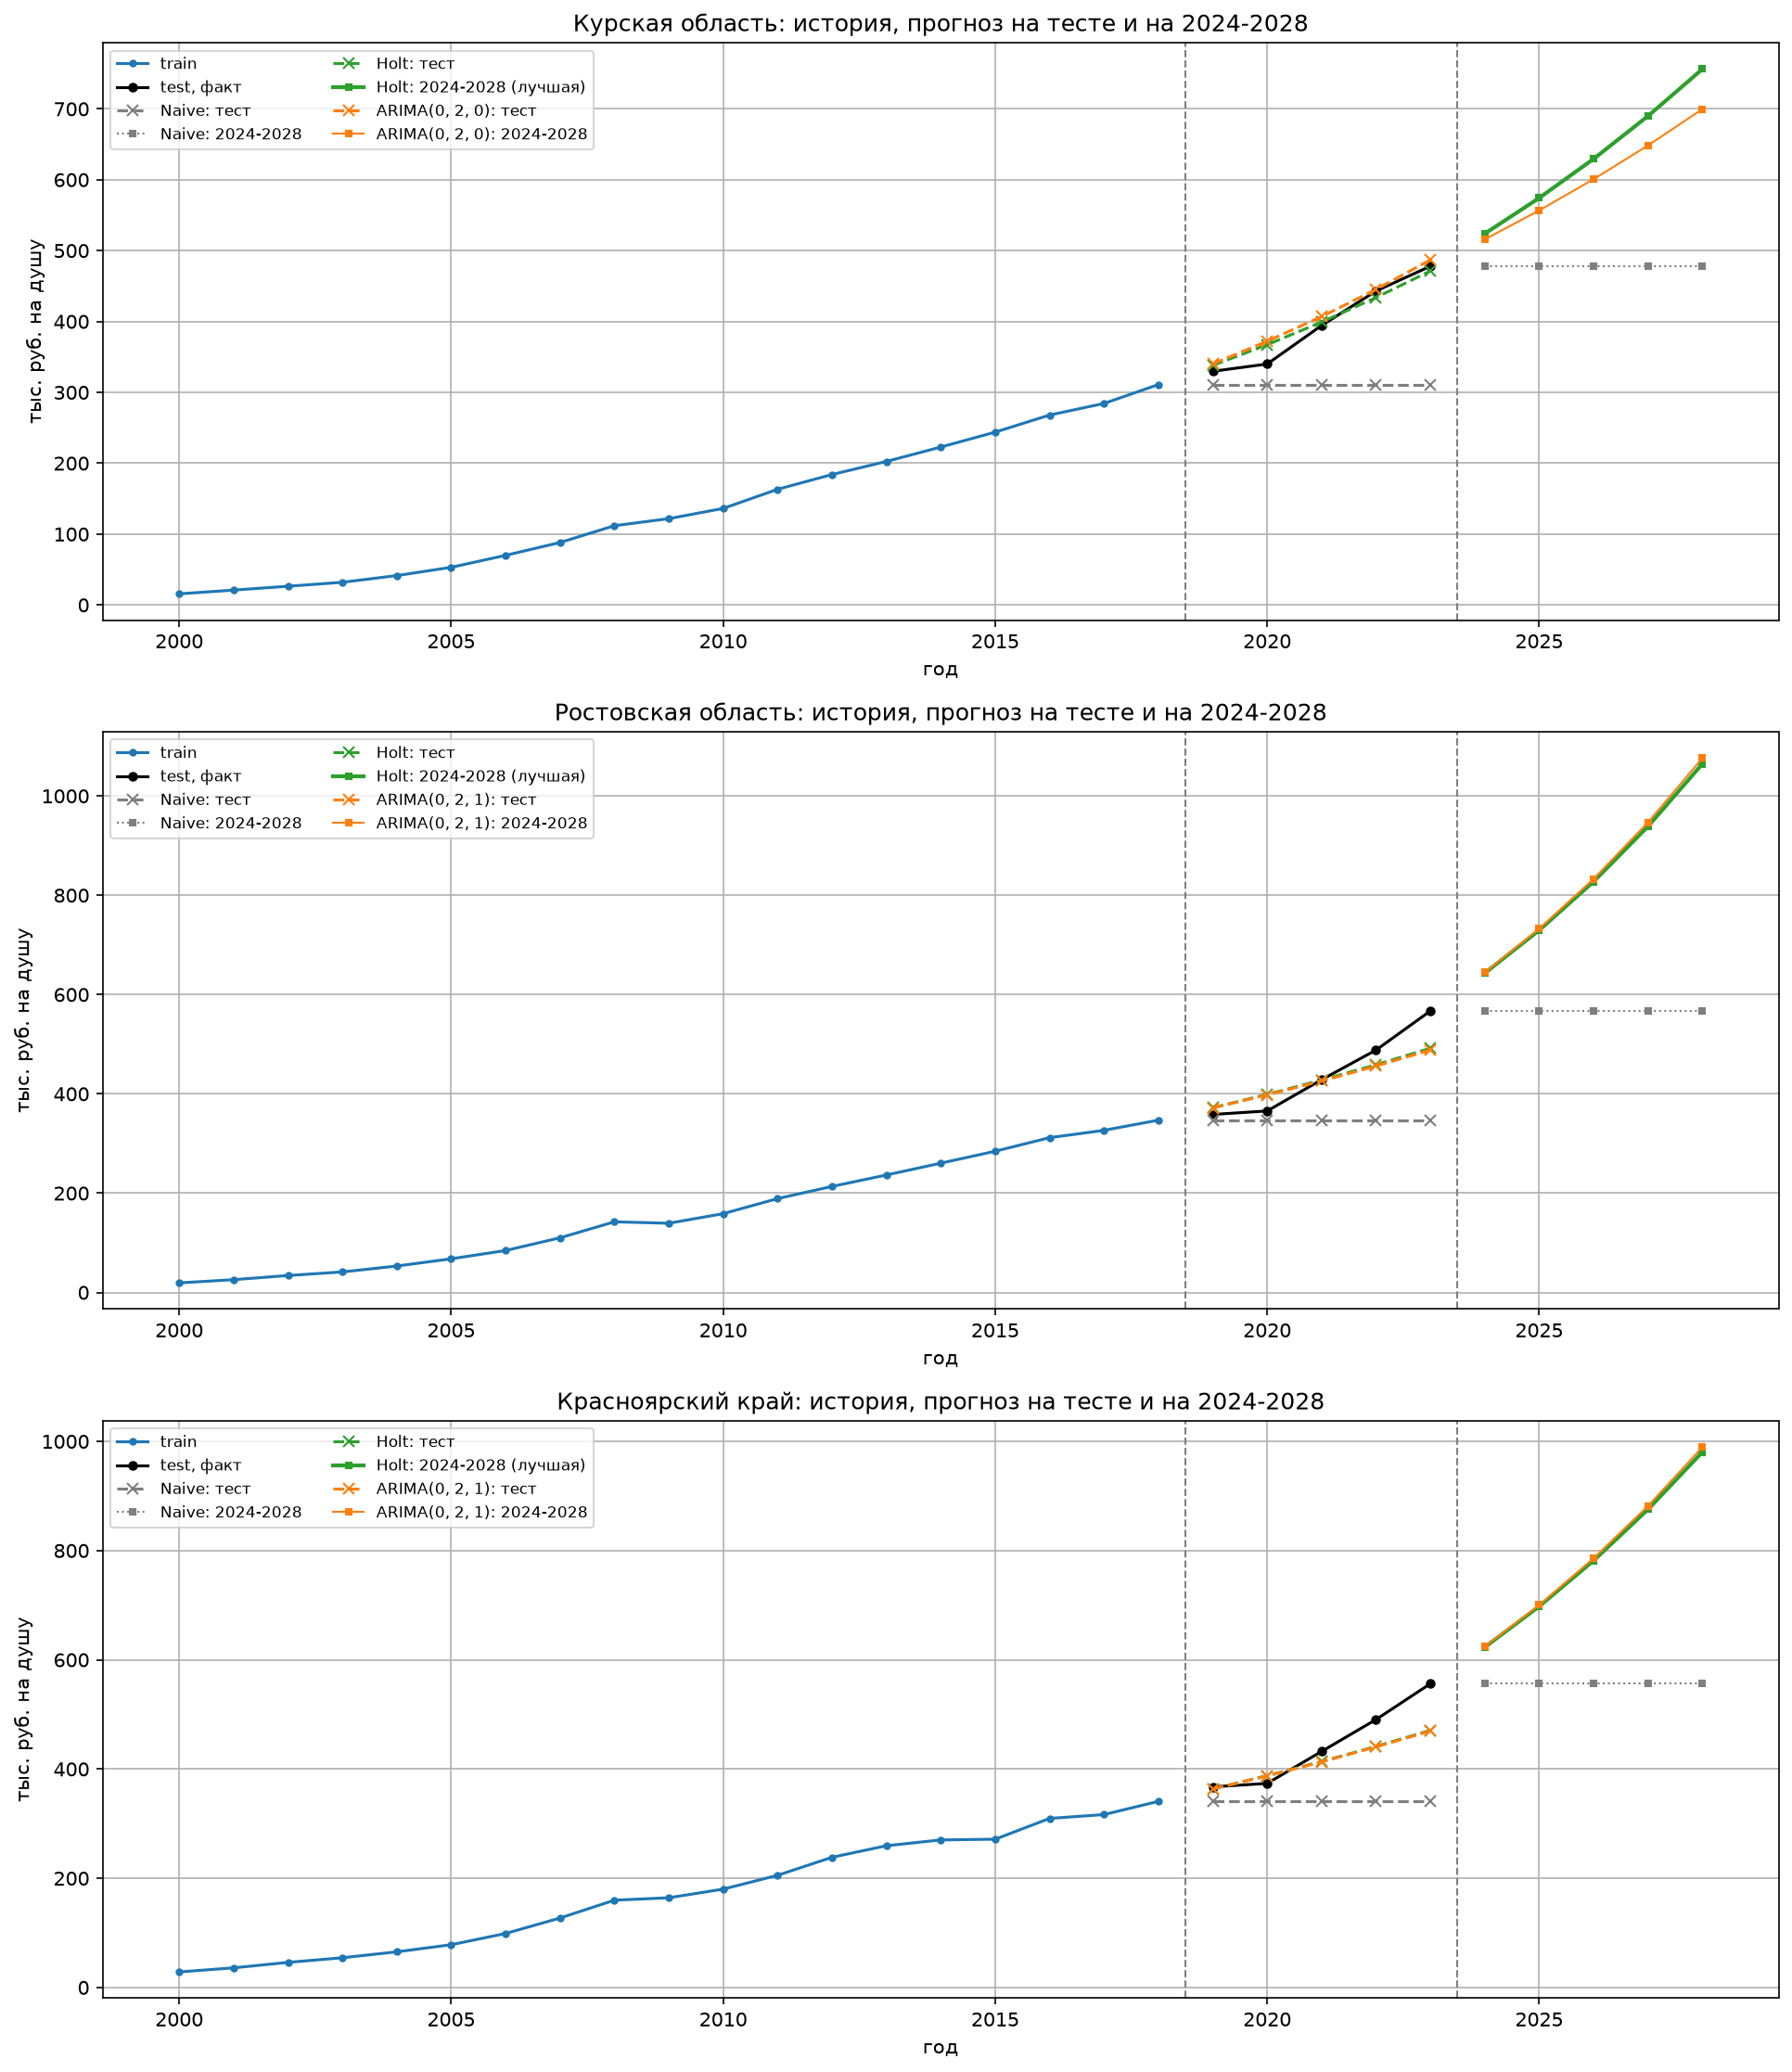
\includegraphics[width=0.92\textwidth]{11_forecasts.png}
    \caption{История, прогноз на тестовой выборке и прогноз на 2024--2028 для трёх моделей}
    \label{fig:forecasts}
\end{figure}

\section{Устойчивость прогноза: expanding window}

Из двух стратегий взял expanding window. Для каждого года t с 2009 по 2023 лучшая модель региона обучается на всех данных 2000..t$-$1 и прогнозирует один шаг вперёд. Обучающая выборка растёт с 9 до 23 точек, а набор прогнозируемых лет фиксирован. По сути это та же кросс-валидация на временном ряду, где фолды идут строго по времени и ряд не перемешивается~\cite{habr-ods,sf-m3}.

По сравнению с rolling здесь не выбрасываются старые наблюдения --- при 24 точках это важно, окно фиксированной длины было бы совсем коротким. 2009 как старт выбран, чтобы в оценку попал кризис 2008--2009. Порядок ARIMA держу тем, что выбран на train, переобучаются только коэффициенты (но лучшей везде всё равно вышел Holt).

\begin{table}[H]
\centering
\caption{Фиксированное разбиение против expanding window (Holt)}
\label{tab:robust}
\small
\begin{tabular}{lrrr}
\toprule
 & Курская & Ростовская & Красноярский \\
\midrule
Fixed split 2019--2023 (прогноз на 1--5 лет): RMSE, руб. & 13\,883 & 39\,596 & 45\,370 \\
Fixed split 2019--2023: MAPE, \% & 3.0 & 6.5 & 6.9 \\
Expanding 2019--2023 (на 1 год): RMSE, руб. & 20\,422 & 27\,241 & 22\,730 \\
Expanding 2019--2023: MAPE, \% & 4.2 & 5.4 & 4.4 \\
\midrule
Expanding, MAPE 2009--2013 (train 9--13 точек), \% & 11.6 & 14.4 & 11.4 \\
Expanding, MAPE 2014--2018 (train 14--18 точек), \% & 1.6 & 2.8 & 6.8 \\
Expanding, MAPE 2019--2023 (train 19--23 точки), \% & 4.2 & 5.4 & 4.4 \\
Expanding, MAPE 2009--2023, \% & 5.8 & 7.6 & 7.5 \\
\bottomrule
\end{tabular}
\end{table}

\begin{figure}[H]
    \centering
    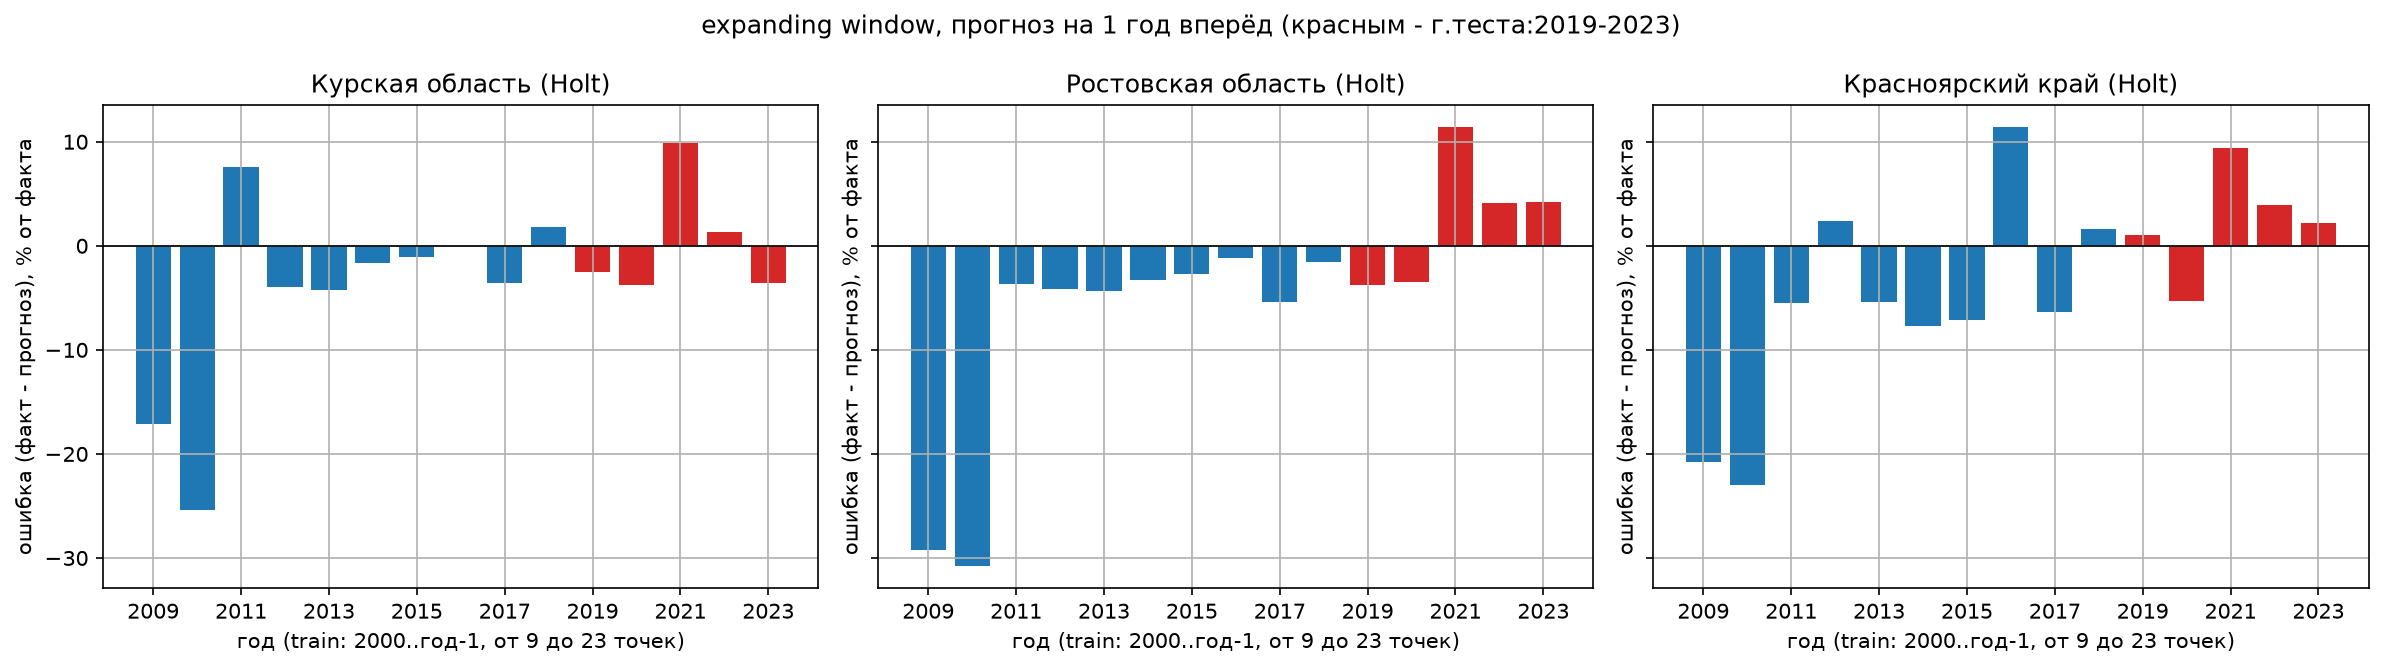
\includegraphics[width=\textwidth]{10_expanding.png}
    \caption{Expanding window: ошибка прогноза на 1 год вперёд по годам, красным --- годы теста}
    \label{fig:expanding}
\end{figure}

На тех же годах 2019--2023 одношаговый прогноз с переобучением даёт MAPE 4.2\%, 5.4\% и 4.4\% против 3.0\%, 6.5\% и 6.9\% на фиксированном разбиении (табл.~\ref{tab:robust}). Для Ростова и Красноярска обновление данных заметно помогает --- модель каждый год подхватывает свежий темп и разгон 2021--2023 уже не пропускает. У Курска наоборот чуть хуже, но там фиксированному прогнозу скорее повезло: ошибки разных знаков компенсировали друг друга, а одношаговый прогноз из провала 2020 честно промахнулся в 2021 (+9.9\%).

Если смотреть по периодам (рис.~\ref{fig:expanding}), видно, как ошибка зависит от накопленных данных. В 2009--2013 MAPE 11--14\% --- в train всего 9--13 точек, и на них пришёлся кризис. В 2014--2018 уже 1.6--2.8\% у Курска и Ростова (6.8\% у Красноярска, его в 2015--2016 качнуло). В 2019--2023 4--5\%. То есть примерно после 14--15 лет истории модель стабилизируется, а дальше ошибка определяется уже шоками, а не длиной ряда. В целом прогноз устойчивый: на последних годах одношаговая ошибка не растёт, и Holt остаётся рабочей моделью при обновлении данных.

\section{Прогноз на 2024--2028}

Для прогноза в будущее модели переобучаются на всём ряде 2000--2023 (порядок ARIMA тот же). Наивный прогноз тут просто равен значению 2023, поэтому в таблицу его не выносил.

\begin{table}[H]
\centering
\caption{Прогноз на 2024--2028, тыс. руб. на душу}
\label{tab:future}
\small
\begin{tabular}{llrrrrrrr}
\toprule
Регион & Модель & Факт 2023 & 2024 & 2025 & 2026 & 2027 & 2028 & \%/год \\
\midrule
Курская область & \textbf{Holt} & 478.0 & 523.9 & 574.3 & 629.4 & 689.9 & 756.1 & 9.6 \\
 & ARIMA(0,2,0) & 478.0 & 515.9 & 556.7 & 600.8 & 648.3 & 699.7 & 7.9 \\
\midrule
Ростовская область & \textbf{Holt} & 567.0 & 643.2 & 729.6 & 827.6 & 938.7 & 1064.8 & 13.4 \\
 & ARIMA(0,2,1) & 567.0 & 644.6 & 732.7 & 832.9 & 946.7 & 1076.2 & 13.7 \\
\midrule
Красноярский край & \textbf{Holt} & 556.3 & 623.1 & 697.9 & 781.7 & 875.5 & 980.5 & 12.0 \\
 & ARIMA(0,2,1) & 556.3 & 624.2 & 700.4 & 785.8 & 881.7 & 989.3 & 12.2 \\
\bottomrule
\end{tabular}
\end{table}

Прогноз продолжает темп последних лет (табл.~\ref{tab:future}). По Holt к 2028 Курская область выходит на 756 тыс. руб. (9.6\% в год), Ростовская на 1065 тыс. (13.4\%), Красноярский край на 980 тыс. (12.0\%). Это скорее верхний сценарий: Holt с $\alpha = 1$ переносит в будущее разгон 2021--2023, у Ростова 13.4\% в год выше даже его фактических 10.3\% за 2019--2023. ARIMA(0,2,0) у Курска даёт более осторожные 700 тыс. (7.9\% в год).

\section{Лучшая модель по регионам}

Во всех трёх регионах лучшая модель --- Holt на логарифме, хотя отрыв от ARIMA минимальный. Объяснение простое: ряды --- это гладкий тренд, наклон которого (темп роста) меняется медленно и без сезонности. Holt как раз и моделирует уровень + наклон, и оба обновляются по свежим данным. На train у всех трёх $\alpha = 1$, то есть уровень просто равен последнему значению, а $\beta$ = 0.42--0.62 --- темп роста подстраивается под последние годы довольно быстро (параметры в табл.~\ref{tab:holt_params} на этапе 6). В логарифме это значит <<продолжаем текущий темп, плавно его обновляя>>. ARIMA(0,2,1) математически почти то же самое, отсюда и почти те же цифры. ARIMA(0,2,0) у Курска --- это <<темп последнего года>>, он шумнее, отсюда чуть больше ошибка.

Типы регионов на выбор модели не повлияли, а вот на точность --- да. Ровный кластер A (Курск) прогнозируется лучше всего (3.0\%), кластеры B и C хуже (6.5--6.9\%), потому что там в тесте случился разгон, который по прошлому не виден.

% ============ ЭТАП 6 ====================
\chapter{Анализ ошибок}

Беру ошибки лучшей модели каждого региона (везде Holt) из expanding window --- прогноз на 1 год вперёд, 2009--2023. Так в разбор попадают 15 лет с кризисами 2009, 2014--2015, 2020 и 2022, а не только 5 лет теста --- иначе <<топ-5>> просто совпал бы со всем тестом. Сортирую по модулю ошибки в процентах. События к годам в таблице подписал по быстрому гуглу, там, где очевидного внешнего события нет, стоит прочерк.

\begin{table}[H]
\centering
\caption{Топ-5 ошибок Holt по каждому региону (прогноз на 1 год вперёд), тыс. руб.}
\label{tab:top5}
\small
\begin{tabular}{lcrrr>{\raggedright\arraybackslash}p{5.6cm}}
\toprule
Регион & Год & Факт & Прогноз & Ошибка, \% & Событие \\
\midrule
Курская & 2010 & 136.2 & 170.8 & $-25.4$ & восстановление после кризиса 2009 \\
 & 2009 & 121.8 & 142.6 & $-17.1$ & мировой финансовый кризис 2008--2009 \\
 & 2021 & 394.4 & 355.2 & +9.9 & восстановление после ковида, ускорение инфляции \\
 & 2011 & 163.2 & 150.8 & +7.6 & -- \\
 & 2013 & 202.5 & 211.1 & $-4.2$ & -- \\
\midrule
Ростовская & 2010 & 158.7 & 207.6 & $-30.8$ & восстановление после кризиса 2009 \\
 & 2009 & 139.4 & 180.1 & $-29.2$ & мировой финансовый кризис 2008--2009 \\
 & 2021 & 428.5 & 379.7 & +11.4 & восстановление после ковида, ускорение инфляции \\
 & 2017 & 326.5 & 344.1 & $-5.4$ & -- \\
 & 2013 & 236.6 & 247.0 & $-4.4$ & -- \\
\midrule
Красноярский & 2010 & 180.1 & 221.5 & $-23.0$ & восстановление после кризиса 2009 \\
 & 2009 & 164.2 & 198.3 & $-20.8$ & мировой финансовый кризис 2008--2009 \\
 & 2016 & 309.5 & 274.2 & +11.4 & стагнация доходов после 2015 \\
 & 2021 & 432.2 & 391.6 & +9.4 & восстановление после ковида, ускорение инфляции \\
 & 2014 & 270.2 & 291.0 & $-7.7$ & падение цен на нефть, санкции, девальвация рубля в конце года \\
\bottomrule
\end{tabular}
\end{table}

\begin{figure}[H]
    \centering
    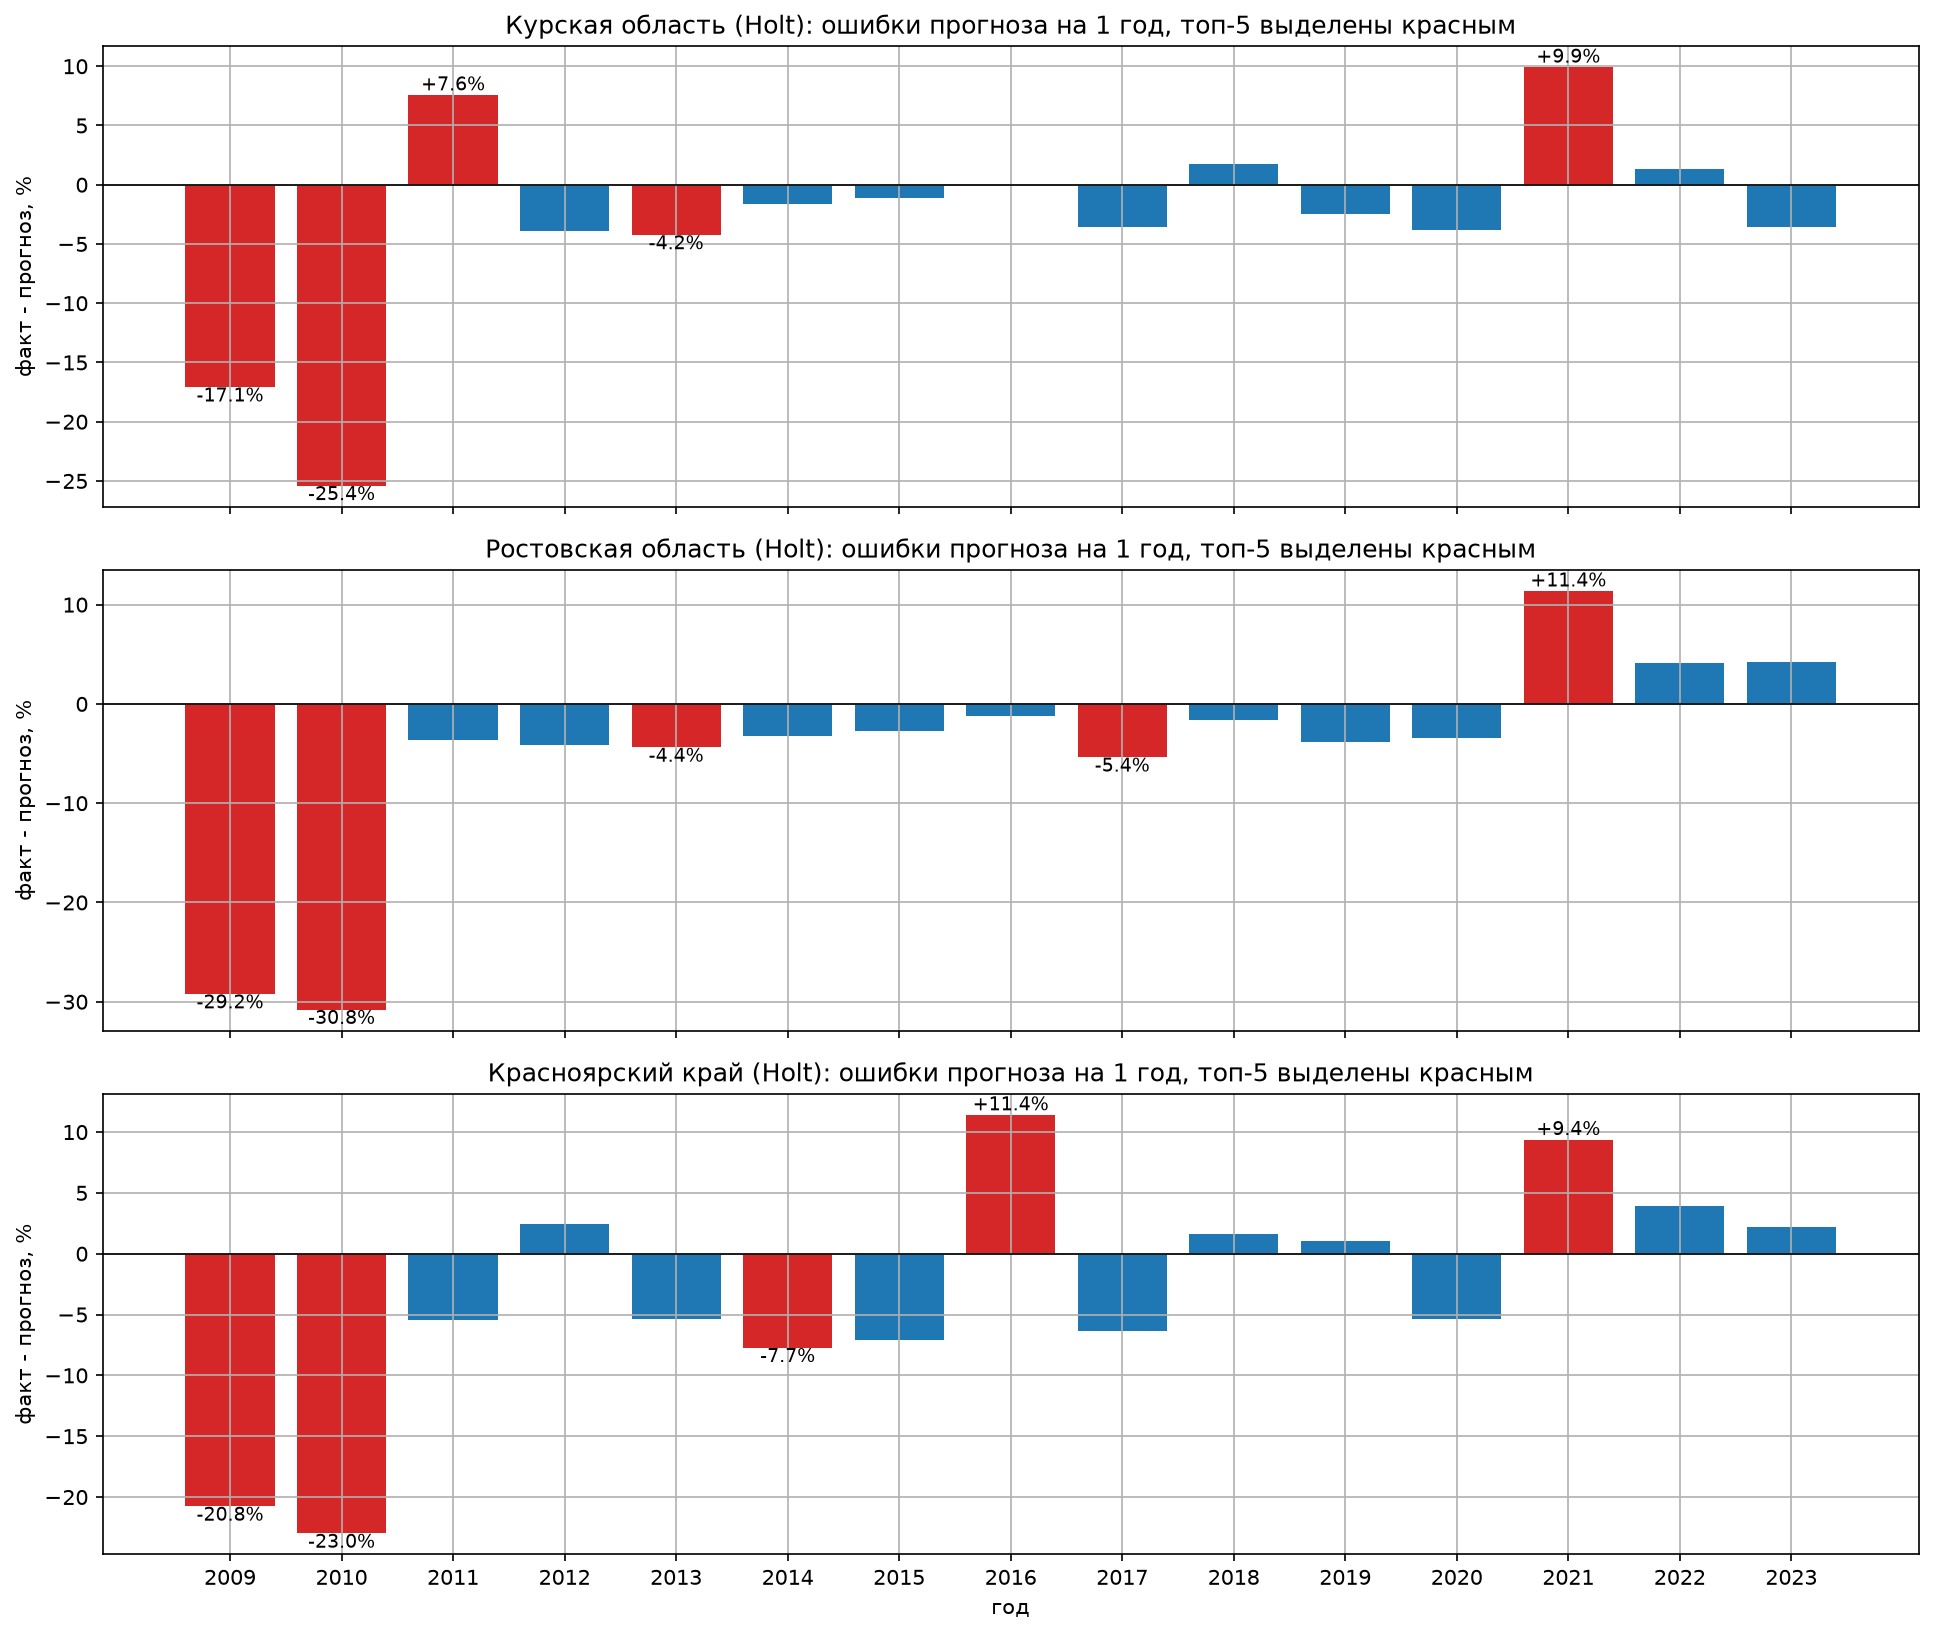
\includegraphics[width=\textwidth]{12_top_errors.png}
    \caption{Ошибки Holt при прогнозе на 1 год вперёд, топ-5 выделены красным}
    \label{fig:top_errors}
\end{figure}

\begin{table}[H]
\centering
\caption{Параметры Holt в зависимости от длины train (темп --- текущий наклон тренда)}
\label{tab:holt_params}
\small
\resizebox{\textwidth}{!}{%
\begin{tabular}{lcccc}
\toprule
Регион & train 2000--2008 & train 2000--2009 & train 2000--2018 & train 2000--2023 \\
\midrule
Курская & $\alpha$=0.00, $\beta$=0.00, 27.6\% & $\alpha$=0.00, $\beta$=0.00, 26.5\% & $\alpha$=1.00, $\beta$=0.62, 8.7\% & $\alpha$=1.00, $\beta$=0.54, 9.6\% \\
Ростовская & $\alpha$=0.00, $\beta$=0.00, 27.7\% & $\alpha$=0.00, $\beta$=0.00, 25.9\% & $\alpha$=1.00, $\beta$=0.42, 7.2\% & $\alpha$=1.00, $\beta$=0.43, 13.4\% \\
Красноярский & $\alpha$=1.00, $\beta$=0.00, 24.1\% & $\alpha$=0.00, $\beta$=0.00, 22.4\% & $\alpha$=1.00, $\beta$=0.43, 6.7\% & $\alpha$=1.00, $\beta$=0.42, 12.0\% \\
\bottomrule
\end{tabular}}
\end{table}

Самые большие промахи у всех трёх регионов --- 2009 и 2010, и это переоценка на 17--31\% (табл.~\ref{tab:top5}, рис.~\ref{fig:top_errors}). Причина тут не только в кризисе. Табл.~\ref{tab:holt_params} показывает, что на 9--10 точках оптимизатор Holt выставил $\beta = 0$ и почти везде $\alpha = 0$, то есть модель выродилась в жёсткую прямую по логарифму, натянутую на бум 2000--2008 (22--28\% роста в год). Кризис 2009 обрушил темп до 9\% у Курска и до $-2\%$ у Ростова, а модель пыталась рисовать докризисный рост. В 2010 ошибка ещё больше, потому что уровень с $\alpha = 0$ вообще не опустился после 2009. Так что 2009--2010 --- это сочетание реального мирового финансового кризиса и слишком короткой истории.

2021 входит в топ у всех: недооценка на 9.4--11.4\%. После провала 2020 модель снизила и уровень, и темп, а в 2021 потребление отскочило на 15--17\% --- отложенный спрос после ограничений плюс ускорение инфляции. Ровно та же логика у Красноярского края в 2016 (+11.4\%): после почти нулевого роста в 2015 модель ждала стагнации, а пришёл отскок на 14\%. Да и Курская область в 2011 (+7.6\%) --- тот же отскок, только после замедления 2009--2010.

Обратная ситуация --- переоценка на входе в спад. Красноярский край в 2014 ($-7.7\%$): рост за год всего 4\%, падение цен на нефть и металлы, девальвация в конце года. Ростовская область в 2017 ($-5.4\%$): реальные доходы населения после 2014 падали несколько лет подряд. Ну и 2013 у Курска и Ростова ($-4.2\%$ и $-4.4\%$), когда экономика замедлялась ещё до санкций.

\textbf{Общая гипотеза получается такая.} Модель экстраполяционная, и косячит она на разворотах: при входе в спад переоценивает, при выходе недооценивает. Сами кризисы --- цены на нефть, курс, инфляция, бюджетные выплаты --- в одномерном ряду никак не видны, поэтому заранее их модель предсказать не может.

% ============ ЭТАП 7 ====================
\chapter{Рекомендации}

Для рекомендаций собрал цифры в одну таблицу (табл.~\ref{tab:rec}): факт 2023, прогноз лучшей модели на 2026 и 2028, разброс между Holt и ARIMA, положение региона относительно медианы 79 регионов (489.1 тыс. руб. в 2023) и типичную ошибку модели из expanding window.

\begin{table}[H]
\centering
\caption{Цифры для рекомендаций}
\label{tab:rec}
\small
\begin{tabular}{lrrr}
\toprule
 & Курская & Ростовская & Красноярский \\
\midrule
Кластер & A & B & C \\
2023, тыс. руб. & 478.0 & 567.0 & 556.3 \\
2023 к медиане регионов, \% & 97.7 & 115.9 & 113.8 \\
Прогноз Holt на 2026, тыс. руб. & 629.4 & 827.6 & 781.7 \\
Прогноз Holt на 2028, тыс. руб. & 756.1 & 1064.8 & 980.5 \\
Holt/ARIMA на 2028: мин--макс, тыс. руб. & 700--756 & 1065--1076 & 981--989 \\
Прогнозный темп 2024--2028, \%/год & 9.6 & 13.4 & 12.0 \\
Фактический темп 2019--2023, \%/год & 9.0 & 10.3 & 10.3 \\
MAPE прогноза на 1 год (expanding 2019--2023), \% & 4.2 & 5.4 & 4.4 \\
\bottomrule
\end{tabular}
\end{table}

\section{Курская область}

Кластер A, 478 тыс. руб. в 2023, 98\% от медианы регионов.

\begin{itemize}
    \item Для бюджетного и социального планирования на 2026 год ориентир --- 600--630 тыс. руб. потребления на душу (ARIMA и Holt). Ошибка модели на 1 год вперёд около 4\%, то есть $\pm$25 тыс. руб. За 23 года у области не было ни одного года снижения, поэтому нижнюю границу коридора можно брать как базовый сценарий.
    \item Номинальный рост 7.9--9.6\% в год по прогнозу --- это примерно уровень инфляции последних лет (быстрый гугл говорит: по Росстату 7.4\% в 2023 и 9.5\% в 2024~\cite{rosstat-cpi}), то есть реального роста потребления почти нет, и область держится чуть ниже медианы (98\%), не догоняя её. Если цель --- выйти выше медианы, нужно опережать прогнозный темп хотя бы на 1--2 п.п. в год.
    \item Модель ничего не знает о событиях 2024 года (эвакуация части жителей, ущерб в районах вдоль границы). Прогноз 524 тыс. на 2024 и 574 тыс. на 2025 лучше считать верхней оценкой и пересчитать сразу, как выйдут фактические данные за 2024.
\end{itemize}

\section{Ростовская область}

Кластер B, 567 тыс. руб. в 2023, 116\% от медианы.

\begin{itemize}
    \item Holt и ARIMA сходятся: 1065--1076 тыс. руб. к 2028 (13.4\% в год). Но это продолжение <<бума>> 2021--2023 (17.2\%, 13.9\%, 16.1\%), а в 2019--2020 темп был всего 3.3\% и 2.0\%. Для планирования я бы брал прогноз как оптимистичный сценарий и держал рядом стресс-сценарий: один год с ростом около 2\%, как в 2009 или 2020, опускает уровень 2028 примерно на 10\%, до 960 тыс.
    \item Область из кластера с просадками, и самые большие промахи из трёх регионов тоже у неё ($-29\%$ в 2009 и $-31\%$ в 2010). Для бизнеса и бюджета это аргумент в пользу запаса около 10\% по ожидаемому потребительскому спросу, а не чёткого планирования.
    \item На тесте модель недооценила 2023 год на 13\%, а при ежегодном переобучении ошибка падает до 5.4\%. Прогноз для этого региона стоит обновлять каждый год по мере выхода данных, а не фиксировать на 5 лет.
\end{itemize}

\section{Красноярский край}

Кластер C, 556 тыс. руб. в 2023, 114\% от медианы.

\begin{itemize}
    \item В 2000 году край был на 63\% выше медианы, а в 2023 только на 14\%. Средний темп 13.8\% против 15.5\% по всем регионам --- отрыв быстро тает. Прогноз 980 тыс. к 2028 (12.0\% в год) по сути закладывает сохранение темпов 2021--2023 (13--16\%). Если край вернётся к своим 2--8\% в год, как в 2017--2020, а остальные регионы продолжат расти около 10\%, к концу горизонта он может уйти ниже медианы.
    \item История ошибок у края связана с сырьевыми циклами: переоценка в 2014 ($-7.7\%$) и недооценка в 2016 (+11.4\%). Прогноз на 2026 (782 тыс.) стоит дополнять сценариями по ценам на металлы и курсу (сам ряд их не учитывает).
    \item Для краевых программ разумно брать не точку, а коридор: на 2025 около 700 тыс. $\pm$5\% (ошибка на год вперёд 4.4\%), а на 2027--2028 уже $\pm$15\% --- столько модель промахнулась к пятому году теста.
\end{itemize}

% ============ ЭТАП 8 ====================
\chapter{Выводы по проекту}

\section{Итоги}

После очистки (выкинуты РФ, 8 федеральных округов, 2 дублирующих агрегата и 6 субъектов с неполным рядом, исправлен выброс у Красноярского края) осталось 79 регионов. K-means на пяти признаках динамики разбил их на три группы: устойчивый быстрый рост без единого года снижения (45 регионов), рост с просадками в кризисы (18, в основном промышленные и сырьевые) и высокий старт с медленным ростом (16, включая Москву). Силуэт у k = 3 не максимальный (0.321 против 0.406 у k = 2), но только при трёх кластерах группы различаются и по устойчивости, и по скорости роста.

Для всех трёх представителей лучшей оказалась модель Holt на логарифме, ARIMA(0,2,0) и ARIMA(0,2,1) почти не отстают, а наивный прогноз проигрывает в 3--7 раз. Тип региона на выбор модели не повлиял, но повлиял на точность: ровный регион из кластера A прогнозируется с MAPE 3\%, регионы из B и C --- 6.5--7\%. Главное, что определяет точность, --- есть ли в горизонте прогноза разворот (кризис или отскок) и насколько длинная история у модели: на 9--10 точках ошибка доходит до 30\%, после 15 лет держится в пределах 2--5\% на шаг.

\section{Ограничения}

Данные в текущих ценах, поэтому прогноз номинальный, и большую его часть составляет инфляция. Ряды короткие (24 точки), так что ADF маломощный, а AIC почти не различает соседние порядки ARIMA. Модели одномерные и экстраполяционные: внешние шоки (нефть, курс, санкции, пандемия, бюджетные выплаты) они не видят и ошибаются как раз на разворотах. Прогноз на 2024--2028 продолжает темп 2021--2023 и в случае замедления инфляции окажется завышенным. Ну и кластеризация сделана по признакам за весь период сразу --- если регион где-то посередине сменил тип динамики, она этого не заметит.

\section{Что можно улучшить}

Дефлировать ряды по региональному ИПЦ и прогнозировать реальное потребление отдельно от инфляции. Добавить экзогенные переменные (ARIMAX с ценой нефти, курсом, инфляцией, доходами населения). Попробовать Holt с затухающим трендом как более осторожный вариант для длинного горизонта. Строить интервальные прогнозы вместо точечных. И использовать иерархию: прогнозы по регионам внутри кластера согласовывать между собой и с прогнозом по РФ.

% ==== ЛИТЕРАТУРА ==========
\begin{thebibliography}{9}

\bibitem{sf-m1}
\textbf{SkillFactory.} Курс <<Временные ряды>>. Модуль 1. Понятие временных рядов.

\bibitem{sf-m2}
\textbf{SkillFactory.} Курс <<Временные ряды>>. Модуль 2. Анализ временных рядов.

\bibitem{sf-m3}
\textbf{SkillFactory.} Курс <<Временные ряды>>. Модуль 3. Моделирование и построение прогнозов.

\bibitem{sf-m4}
\textbf{SkillFactory.} Курс <<Временные ряды>>. Модуль 4. Экспоненциальное сглаживание.

\bibitem{sf-m5}
\textbf{SkillFactory.} Курс <<Временные ряды>>. Модуль 5. Модели ARIMA и их расширения.

\bibitem{habr-ods}
\textbf{Open Data Science.}
Открытый курс машинного обучения. Тема 9. Анализ временных рядов с помощью Python. --- Хабр, 2017. ---
\url{https://habr.com/ru/companies/ods/articles/327242/}.

\bibitem{habr-arima}
\textbf{Ermak\_Marina.}
Временные ряды и ARIMA: Как предсказывать будущее без хрустального шара. --- Хабр, 2024. ---
\url{https://habr.com/ru/articles/821231/}.

\bibitem{rosstat-cpi}
\textbf{Росстат.}
Индексы потребительских цен. ---
\url{https://rosstat.gov.ru/statistics/price}.

\end{thebibliography}

\end{document}
